% !TeX spellcheck = en_GB
\documentclass[main.tex]{subfiles}

\begin{document}
\chapter{Experiments and Discussion}
\lhead{Experiments and Discussion}
\label{chap:discussion}

\section{What Is Going on in the Pretraining?}
\label{sec:pretrainpls}
In order to investigate what affects pretraining effectiveness, several ablation studies are performed.
Unless stated otherwise, the main hyperparameters from Table \ref{tab:pretrain-hyper} are used, but with 50 epochs due to limited compute.
The experiments were trained primarily on a $ 1\times$A100 configuration.
Due to its negative effect on runtime on A100's (see Figure \ref{fig:runtime}), AMP is not used for any of the following experiments.
\subsection{The Parameter Population}
The first model analysis is a global view of the DaLUKE parameters.
Figure \ref{fig:weight-dist} shows the model parameter value distribution before and after pretraining divided by whether or not a given parameter was initialized from da-BERT.
\begin{figure}[H]
    \centering
    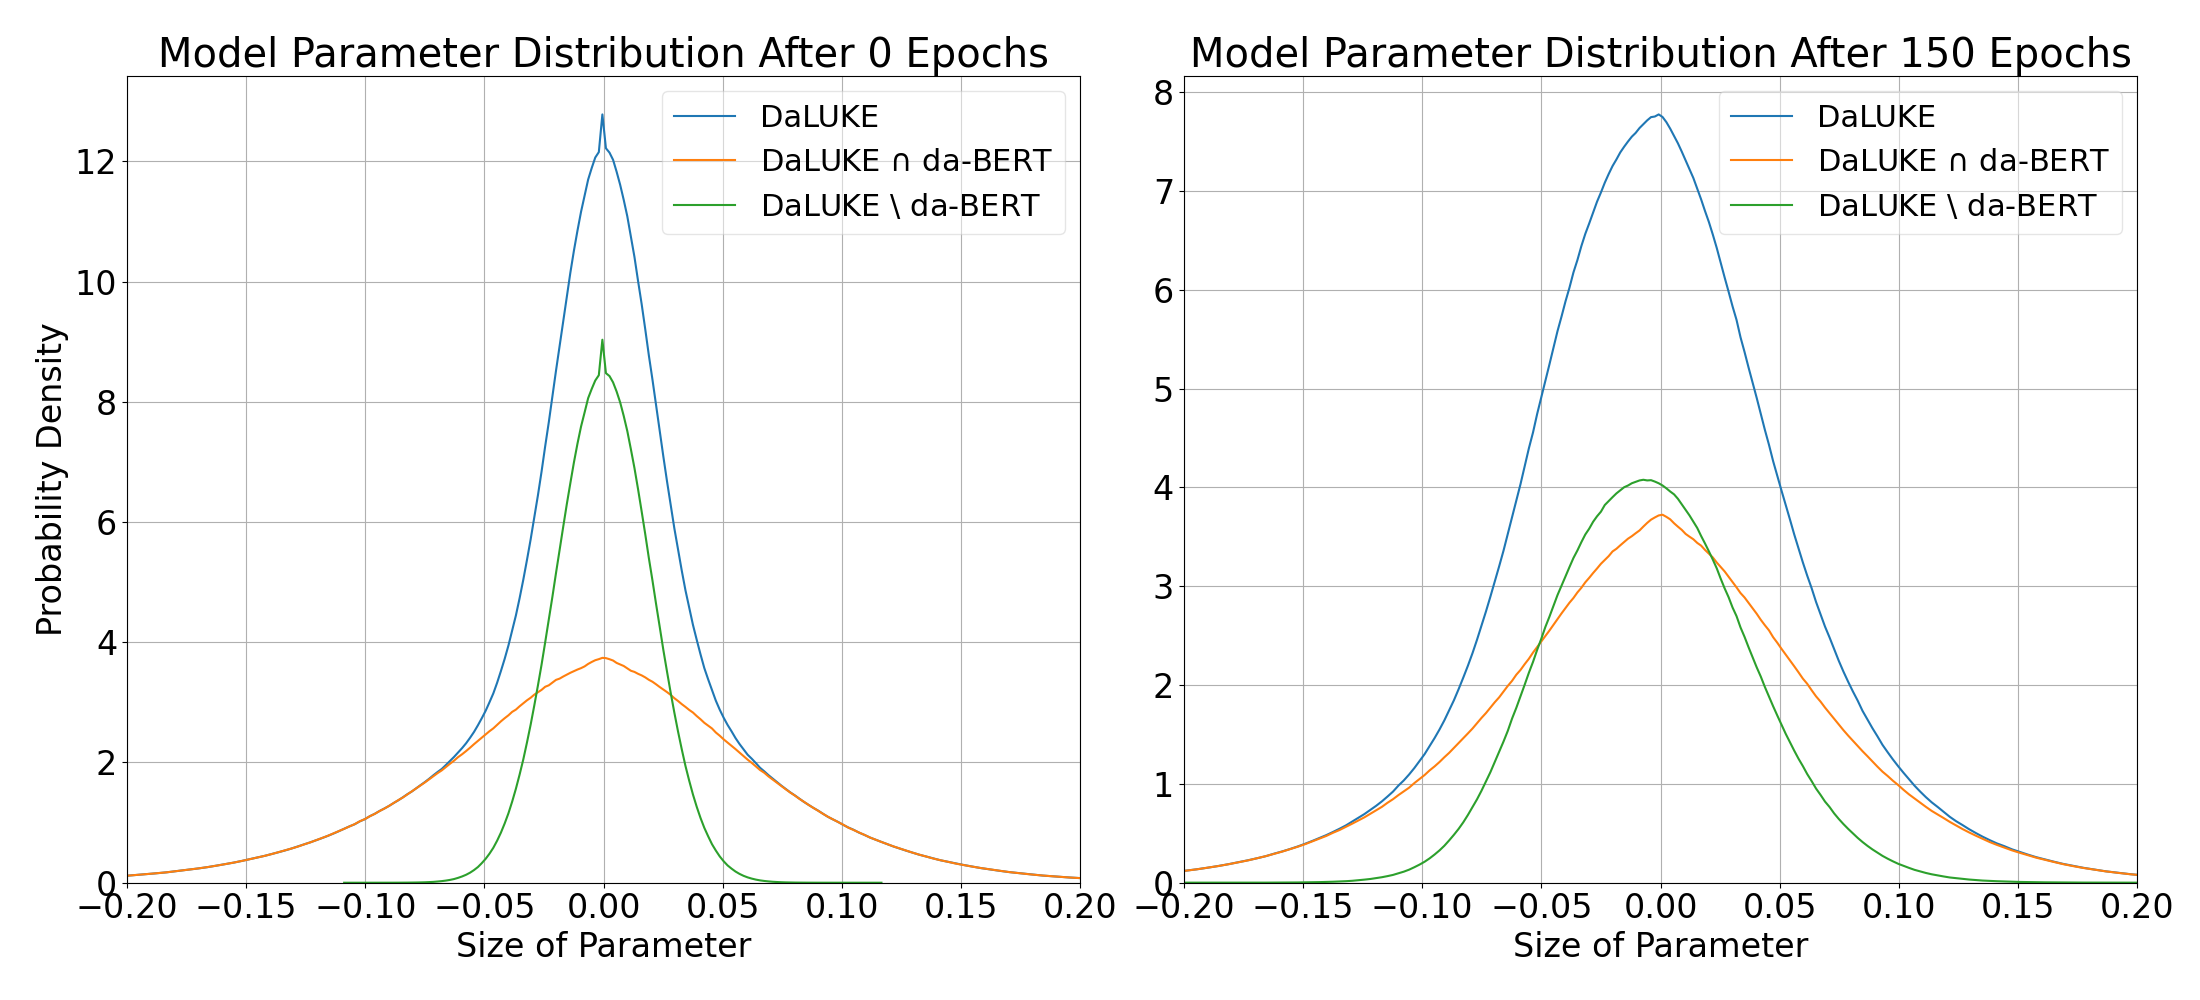
\includegraphics[width=\textwidth]{weights}
    \caption{
        The parameter distribution before and after pretraining, including the decoder.
        DaLUKE $ \cap $ da-BERT (orange) refers to the parameters that transferred from da-BERT, including the query matrices in the entity-aware self-attention.
        DaLUKE $ \backslash $ da-BERT (green) are the remaining parameters.
        These are made up of the entity embeddings (58 million parameters) and the entity decoder (58 million parameters).
        In total, the model has 273 million parameters.
        Note that DaLUKE $ \cap $ da-BERT and DaLUKE $ \backslash $ da-BERT are not full probability densities but rather subsets that together make up the DaLUKE graph, which is a full probability density.
    }
    \label{fig:weight-dist}
\end{figure}\noindent
Two observations stand out:
Firstly, DaLUKE exclusive parameters, which consist of entity embeddings and the entity part of the decoder, are spread out.
This includes the notable peak that comes from biases and layer normalizations being initialized to 0.
Secondly, the shared parameters are more or less unchanged in their distribution.
This makes sense, as they are already trained, and so further training on similar data with a similar task should not result in any significant change.
Furthermore, all parameters from da-BERT (barring the three sets of DaLUKE exclusive query matrices) are not changed for the first half of training.
When they are finally unlocked, both the loss and learning rate have dropped significantly, resulting in less change.

It is noted that the new DaLUKE parameters after training forms a distribution appearing very close to Gaussian.
These are mostly made up of entity embeddings which are subjected to layer normalizations which we suspect to be influential on this shape.

\subsection{Effect of More Pretraining}
\label{subsec:effmore}
The goal of the pretraining is to infuse the model with general language understanding, but it is not immediately clear how to measure such an abstract concept.
The simplest idea is naturally the loss and by extension the top $ k $ accuracies, but this approach is not exempt of issues:
Without a validation set, overfitting can be disguised as improvement (especially on small datasets), or perhaps decreases in loss come from the decoder part of the masked language modelling, which is irrelevant to downstream tasks.

One way to glimpse into the pretraining black box is to observe the performance of downstream language tasks on a number of checkpoints produced during the pretraining.
Such a checkpoint was produced just after model initialization and following that at roughly every fifth epoch for a total of 32 checkpoints.
At every checkpoint, fine-tuning and evaluation on DaNE was performed using the hyperparameters from Table \ref{tab:baseline-hyper}.
The result is shown in Figure \ref{fig:running}.
\begin{figure}[H]
    \centering
    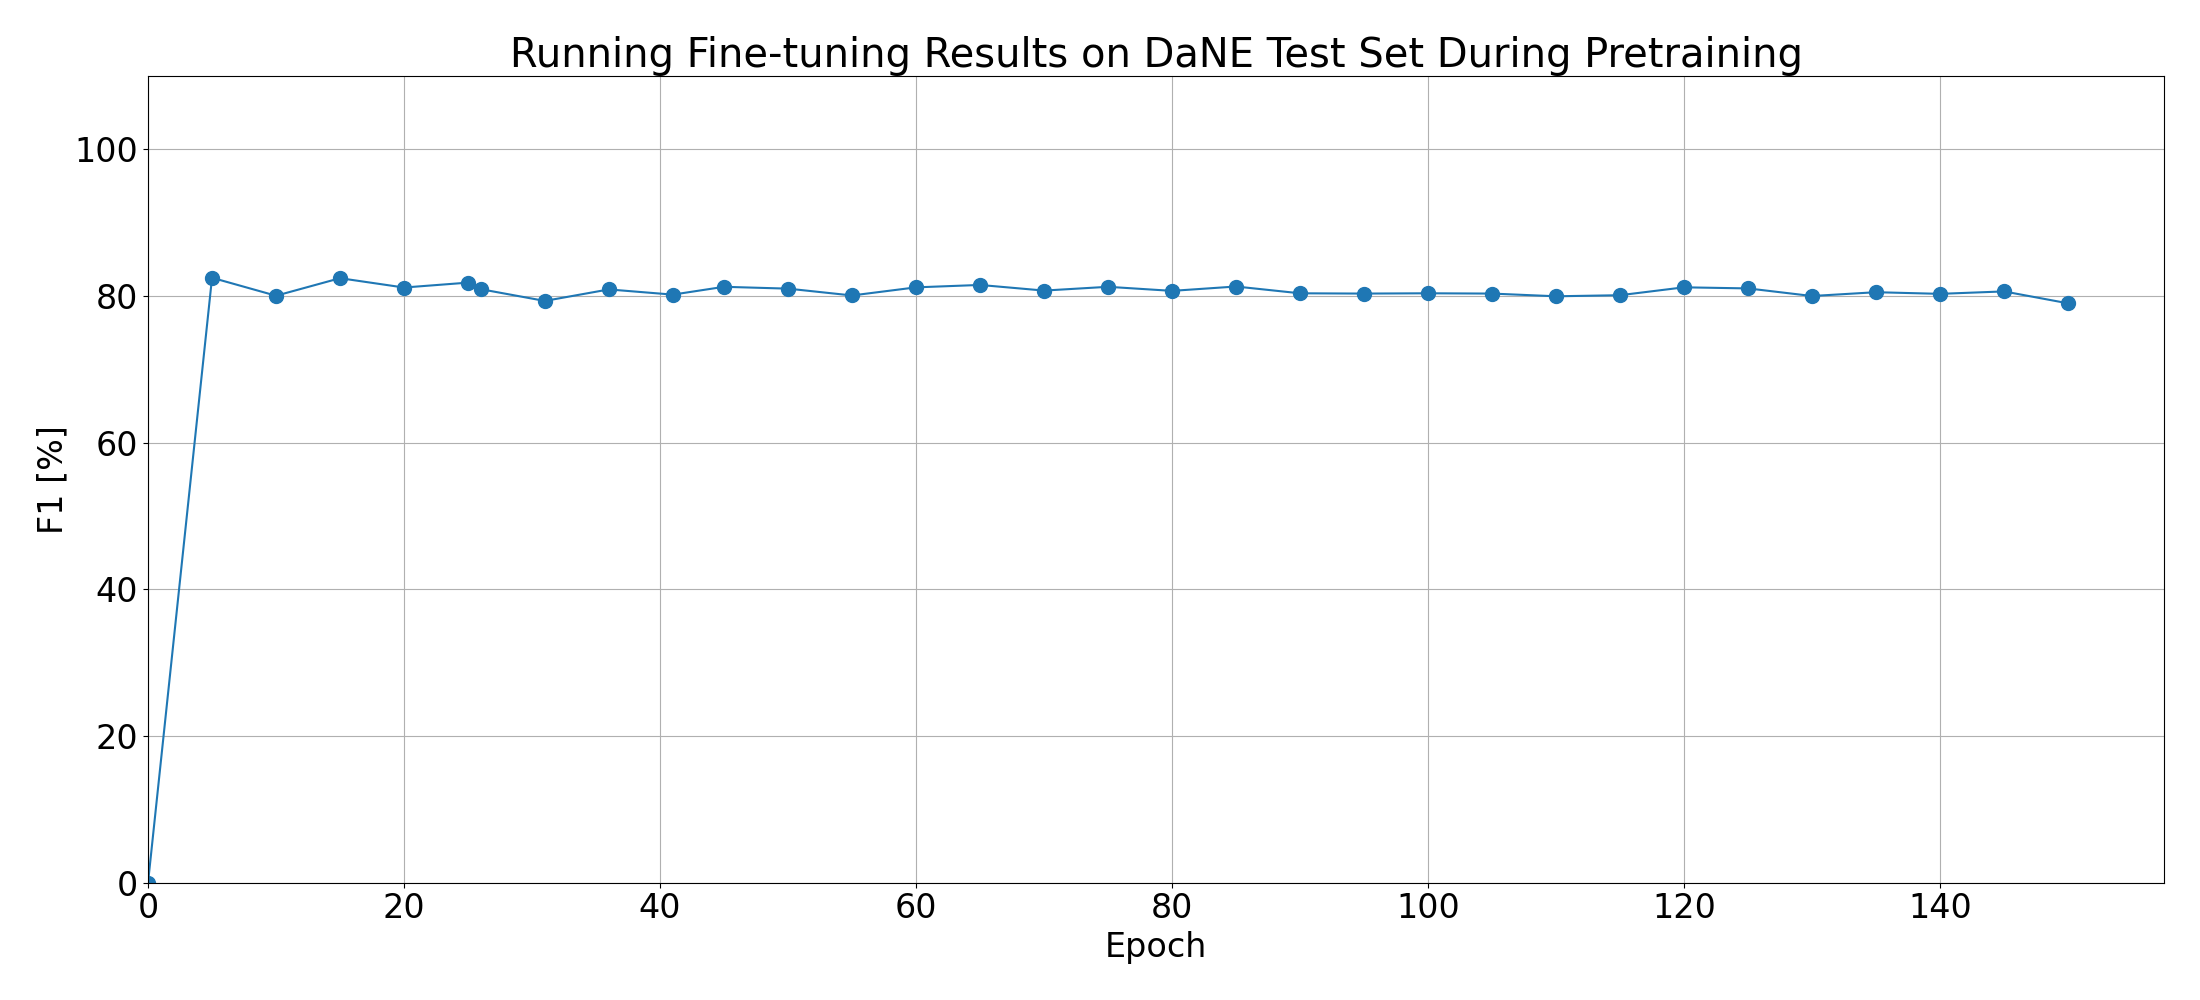
\includegraphics[width=.9\textwidth]{running}
    \caption{Fine-tuning results on DaNE using different pretraining checkpoints.}
    \label{fig:running}
\end{figure}\noindent
This result shows that pretraining definitely is necessary to get good performance on NER.
Somewhat surprisingly, however, after five epochs -- or maybe even less -- additional pretraining does not improve downstream results even slightly.
In fact, the curve almost perfectly mirrors the masked subword accuracy form Figure \ref{fig:pretrain-acc}, indicating that the model primarily relies on its BERT subset for NER.

It must be noted that NER is just one downstream task and that other such tasks may see more benefit from additional pretraining.
However, another explanation may be more probable:
That the Danish Wikipedia is so small that it only takes a few epochs for DaLUKE to learn what it can from it -- especially given that Wikipedia made up an albeit small but still notable part of da-BERT's training data, so it already has been seen \cite{botxo2019dabert}.
That would also help explain the much faster convergence of subword accuracy compared to entity accuracy.
The pretraining dataset only has a little over 100 million subword tokens (see Table \ref{tab:metadata}) and 7.2 million entity annotations -- not exactly much for a model with 270 million parameters and an architecture with a well-known near insatiable thirst for data.

\subsection{Baseline}
For a baseline model, the main model is retrained using only 50 epochs, but otherwise using the same hyperparameters, shown in Table \ref{tab:pretrain-hyper}.
This allows for a comparison to a number of ablation studies where compute resources did not allow a full 150 epoch pretraining.

The final results of this pretraining are summarized in Table \ref{tab:baseline-mlm} with the accuracy development shown on Figure \ref{fig:baseline-acc}.

\begin{table}[H]
    \centering
    \small
    \begin{tabular}{l|l|cccccc}
        Model                           & Top $k$ accuracy [\pro]  & $k=1$  & $k=3$ & $k=5$ & $k=10$ & $k=25$ & $k=50$\\\hline
        \multirow{2}{*}{Baseline}       & Masked words             & 24.2  & 30.9 & 34.4 & 39.7  & 47.7  & 53.6 \\
                                        & Masked entities          & 28.8  & 39.0 & 50.6 & 50.6  & 59.6  & 66.3
    \end{tabular}
    \caption{
        The top $k$ accuracy of the baseline model in the 50'th and last epoch.
    }
    \label{tab:baseline-mlm}
\end{table}\noindent
% 2021-06-11 19:37:14.230    INFO        K=1
%                                        Word:   24.231
%                                        Entity: 28.800
% 2021-06-11 19:37:14.235    INFO        K=3
%                                        Word:   30.937
%                                        Entity: 39.009
% 2021-06-11 19:37:14.238    INFO        K=5
%                                        Word:   34.371
%                                        Entity: 43.843
% 2021-06-11 19:37:14.242    INFO        K=10
%                                        Word:   39.701
%                                        Entity: 50.637
% 2021-06-11 19:37:14.245    INFO        K=25
%                                        Word:   47.708
%                                        Entity: 59.567
% 2021-06-11 19:37:14.249    INFO        K=50
%                                        Word:   53.619
%                                        Entity: 66.324
\begin{figure}[H]
    \centering
    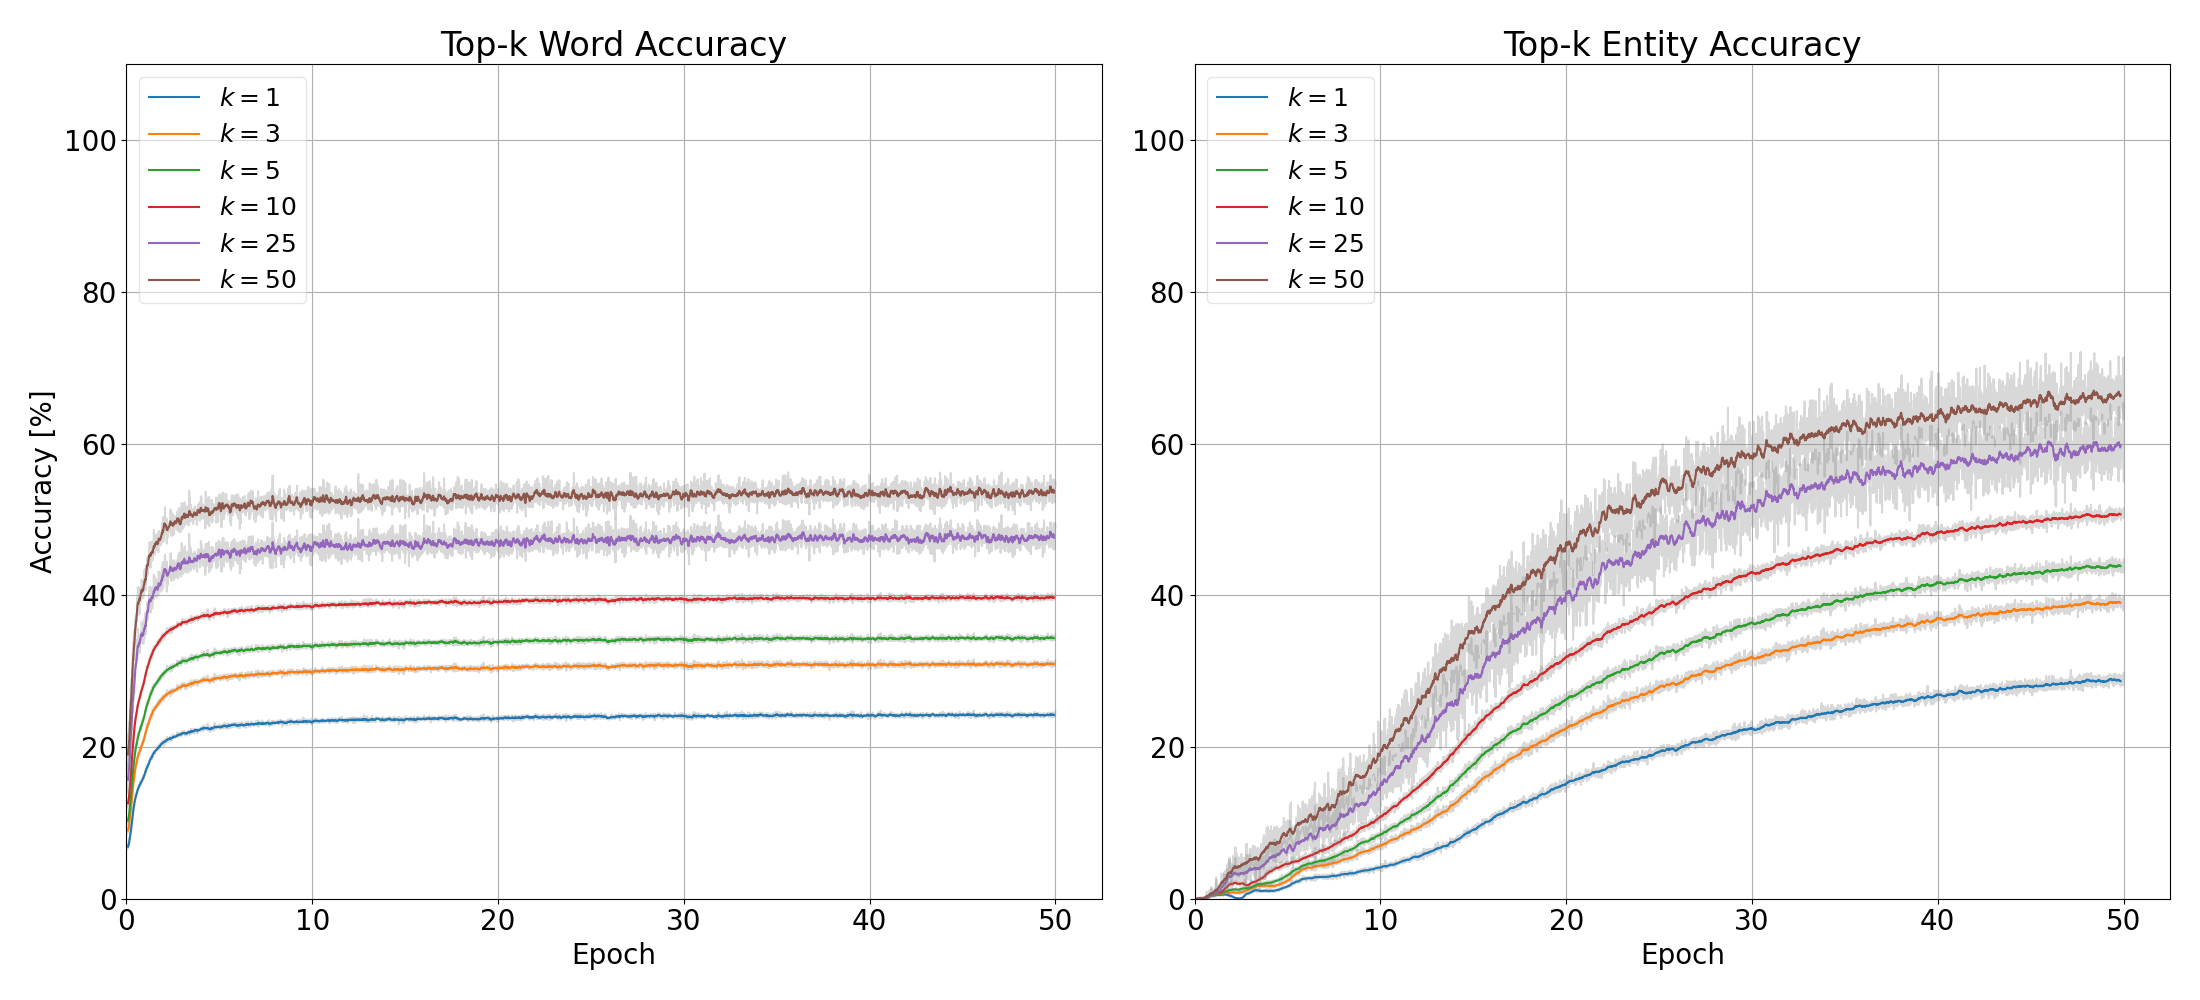
\includegraphics[width=\textwidth]{baseline-acc}
    \caption{Baseline masked language and masked entity accuracy throughout pretraining.
    All curves are smoothed using a rolling average.}
    \label{fig:baseline-acc}
\end{figure}\noindent
The model is afterwards fine-tuned for named entity recognition on DaNE following the approach described in Section~\ref{sub:fine-tune-ner} and the following hyperparameters, non-systematically selected:
\begin{table}[H]
    \centering
    \small
    \begin{tabular}{l|r}
        Parameter  &    \jl{Value}\\\hline
        Epochs     & 10\\
        Batch size &    16\\
        Peak learning rate & $2\ctp{-5}$\\
        LR warmup steps proportion & $ 6\pro $\\
        Dropout (pretrained model) & $ 0.1 $\\
        Dropout (final, linear layer) & $ 0.025 $\\
        Weight decay & $ 0.05 $\\
        Loss weighting & No
    \end{tabular}
    \caption{Hyperparameters for baseline fine-tuning experiment and the following ablation experiments.}\label{tab:baseline-hyper}
\end{table}\noindent
This resulted in the following performance on the DaNE test dataset.
\begin{table}[H]
    \centering
    \small
    \begin{tabular}{l|ccccc|c|c}
        \multirow{2}{*}{Model}  & \multicolumn{5}{c|}{F1 [\pro]} & Precision [\pro]               & Recall [\pro]               \\
                            & Avg. & LOC & PER & ORG & MISC      & Avg.                           & Avg.                         \\ \hline
    Baseline                & 82.4 $\pm 3$ &89.5&92.9&74.4&68.8      & 86.7                          & 78.4
    \end{tabular}
    \caption{The baseline fine-tuning results}
    \label{tab:summary}
\end{table}\noindent
The results of the baseline experiment together with the following experiments are also shown together in a final overview at Section \ref{subsec:preoverview}.
 % 2021-06-11 19:53:46.665    INFO                      precision    recall f1-score   support

 %                                                LOC     0.8958    0.8958   0.8958        96
 %                                               MISC     0.7872    0.6116   0.6884       121
 %                                                ORG     0.8372    0.6708   0.7448       161
 %                                                PER     0.9140    0.9444   0.9290       180

 %                                          micro avg     0.8673    0.7849   0.8241       558
 %                                          macro avg     0.8586    0.7807   0.8145       558
 %                                       weighted avg     0.8612    0.7849   0.8180       558

\subsection{Entity-aware Self-attention}
\label{subsec:selfatt}
The entity-aware self-attention mechanism, one of Yamada et al.'s key contributions to the transformer, was used for our pretraining task.
An experiment using the traditional attention, which does not discrimante between word and entity tokens, was performed.
% is the addition of query matrices for relations between entities and words.
% They do not use these extra matrices in the pretraining but instead let them be learned during downstream tasks, initializing them to the word-to-word matrices of RoBERTa.
% They perform ablation studies on multiple datasets, showing an improvement in every case over original attention.
% \cite{yamada2020luke}

% These results suggest that training the extra query matrices in the pretraining also might have a positive impact.
% For this reason, entity-aware self-attention has been used here for all pretrainings bar this one, where its effects on pretraining is investigated.

This model yields worse results than the main model on the pretraining task shown on Table~\ref{tab:bert-attention-mlm}.
\begin{table}[H]
    \centering
    \small
    \begin{tabular}{l|l|cccccc}
        Model                               & Top $k$-accuracy [\pro]  & $k=1$  & $k=3$ & $k=5$ & $k=10$ & $k=25$ & $k=50$\\\hline
        \multirow{2}{*}{BERT attention}     & Masked words             & 20.6  & 26.3 & 29.4 & 34.6  & 42.4  & 48.7 \\
                                            & Masked entities          & 12.3  & 21.0 & 25.7 & 32.8  & 42.9 & 51.5
    \end{tabular}
    \caption{
        The top $k$ accuracy of the pretrained model trained without entity-aware self-attention in the 50'th and last epoch.
    }
    \label{tab:bert-attention-mlm}
\end{table}\noindent
After fine-tuning, the following results were achieved:

\begin{table}[H]
    \centering
    \small
    \begin{tabular}{l|ccccc|c|c}
        \multirow{2}{*}{Model}  & \multicolumn{5}{c|}{F1 [\pro]} & Precision [\pro]               & Recall [\pro]               \\
                            & Avg. & LOC & PER & ORG & MISC      & Avg.                           & Avg.                         \\ \hline
    BERT attention          & 79.6 $\pm 3$ & 85.8 & 92.8 & 70.9 &   64.8      & 84.5                          & 75.2
    \end{tabular}
   \caption{The fine-tuning results of the traditional attention experiment.}
    \label{tab:bertatt}
\end{table}\noindent
From the lower NER and masked language performances, it is concluded that this mechanism explicitly modeling the difference between the two token domains is an important part of the DaLUKE results.

% 2021-06-12 12:21:29.881    INFO                      precision    recall  f1-score   support

%                                                 LOC     0.7191    0.6667    0.6919        96
%                                                MISC     0.6585    0.4463    0.5320       121
%                                                 ORG     0.6364    0.2609    0.3700       161
%                                                 PER     0.7563    0.5000    0.6020       180

%                                           micro avg     0.7022    0.4480    0.5470       558
%                                           macro avg     0.6926    0.4685    0.5490       558
%                                        weighted avg     0.6941    0.4480    0.5354       558

\subsection{Dataset Augmentation}
\label{subsec:dataexp}
A key addition to the pretraining pipeline was the addition of extra entity annotations not already in the Wikipedia articles themselves using pattern matching as explained in Section~\ref{subsec:entaug}.
This resulted in a 47\pro\ growth in the number of annotations as shown in Table~\ref{tab:metadata}.
While it was argued that it should improve performance, it was all theoretical.
Therefore, this effect of the augmentation is investigated by pretraining a model with the original data for 50 epochs and same hyperparameters as the main experiment.

The pretraining terminated to the following performance.

\begin{table}[H]
    \centering
    \small
    \begin{tabular}{l|l|cccccc}
        Model                               & Top $k$-accuracy [\pro]  & $k=1$  & $k=3$ & $k=5$ & $k=10$ & $k=25$ & $k=50$\\\hline
        \multirow{2}{*}{No data aug.}       & Masked words             & 25.3  & 32.2 & 35.6 & 40.9  & 48.8  & 54.6 \\
                                            & Masked entities          & 34.0  & 42.9 & 47.2 & 53.5  & 62.3 & 68.8
    \end{tabular}
    \caption{
        The top $k$ accuracy of the pretrained model trained without dataset augmentation in the 50'th and last epoch.
    }
    \label{tab:old-data-mlm}
\end{table}\noindent
At a first glance, these masked language modeling results that strictly dominate the numbers for the baseline seem to suggest that the dataset augmentation was ill-advised.
There is, however, a large issue (apart from the obvious problem of judging a model by its performance on the training dataset) with the metric in this case:
The dataset augmentation also changed the benchmark itself as the masking task of the baseline model also includes automatically annotated, and thus somewhat dubious, entity links.
This can explain the clear gain in entity masking performance of this experiment.
Whether this explanation has any merit in explaining the increased word accuracy found in this ablation study is less clear to us and relates to the model synergy effects in this joint task.

% 2021-06-11 19:38:23.333    INFO        K=1
%                                        Word:   25.260
%                                        Entity: 34.015
% 2021-06-11 19:38:23.340    INFO        K=3
%                                        Word:   32.155
%                                        Entity: 42.846
% 2021-06-11 19:38:23.345    INFO        K=5
%                                        Word:   35.601
%                                        Entity: 47.212
% 2021-06-11 19:38:23.351    INFO        K=10
%                                        Word:   40.926
%                                        Entity: 53.520
% 2021-06-11 19:38:23.356    INFO        K=25
%                                        Word:   48.776
%                                        Entity: 62.258
% 2021-06-11 19:38:23.361    INFO        K=50
%                                        Word:   54.617
%                                        Entity: 68.818
As a more unbiased benchmark, this model was fine-tuned on the DaNE dataset using the hyperparameters at Table~\ref{tab:baseline-hyper} resulting in the following performance:
\begin{table}[H]
    \centering
    \small
    \begin{tabular}{l|ccccc|c|c}
        \multirow{2}{*}{Model}  & \multicolumn{5}{c|}{F1 [\pro]} & Precision [\pro]               & Recall [\pro]               \\
                            & Avg. & LOC & PER & ORG & MISC      & Avg.                           & Avg.                         \\ \hline
    No data aug.            & 83.0 $\pm 3$&84.4&95.1&76.4&72.1      & 85.4                          & 80.8
    \end{tabular}
    \caption{The fine-tuning results of the dataset augmentation pretraining experiment.}
    \label{tab:dataaug}
\end{table}\noindent
% 2021-06-11 16:08:34.724    INFO                      precision    recall  f1-score   support

%                                                 LOC     0.8155    0.8750    0.8442        96
%                                                MISC     0.7500    0.6942    0.7210       121
%                                                 ORG     0.8214    0.7143    0.7641       161
%                                                 PER     0.9711    0.9333    0.9518       180

%                                           micro avg     0.8542    0.8082    0.8306       558
%                                           macro avg     0.8395    0.8042    0.8203       558
%                                        weighted avg     0.8532    0.8082    0.8291       558
The ablation study gets substantially higher recall than the baseline resulting in a higher micro average F1 score on the NER task, though the baseline outperforms in precision.

All in all, these benchmarks cannot be used to support our theorized problem of of false negatives in the volunteer-produced annotations or at least not that it is mitigated by this augmentation approach.
If anything, the addition of automatic pattern-matched annotations worsened the performance slightly.

As the addition of these $47\pro$ bronze standard annotations did not directly stop the learning, we still propose such automated annotation  as an avenue for further development of DaLUKE.
\subsection{Impact of Danish BERT}
\label{subsec:dabertexp}
As described in section \ref{sec:LUKE}, many of the weights are initialized from a base transformer.
This transfer learning method ideally gives DaLUKE all the contextual language understanding of da-BERT.
In order to test this hypothesis, a pretraining is conducted without initializing the weights to da-BERT.

\begin{table}[H]
    \centering
    \small
    \begin{tabular}{l|l|cccccc}
        Model                                 & Top $k$ accuracy [\pro]  & $k=1$  & $k=3$ & $k=5$ & $k=10$ & $k=25$ & $k=50$\\\hline
        No transfer & Masked words             & 47.9  & 59.3 & 63.9 & 69.8  & 76.5 & 81.0 \\
        learning                                      & Masked entities          & 81.7  & 87.2 & 88.9 & 90.9  & 93.2 & 94.6
    \end{tabular}
    \caption{
        The top $K$ accuracy of the pretrained model trained without initializing weights from da-BERT in the 50'th and last epoch.
    }
    \label{tab:nobert-mlm}
\end{table}\noindent
It is immediately clear from Table \ref{tab:nobert-mlm} that this model performs noticeably better at both the masked word and masked entity tasks than other models so far.
That is despite even starting from 0 in the masked word task (see Figure \ref{fig:nobert-acc}).
Because of this, good NER performance could reasonbly be expected.
This did not happen - in fact, results were much worse than the baseline.
% 2021-06-12 12:20:54.130    INFO                      precision    recall  f1-score   support

%                                                 LOC     0.7281    0.8646    0.7905        96
%                                                MISC     0.6514    0.5868    0.6174       121
%                                                 ORG     0.7841    0.4286    0.5542       161
%                                                 PER     0.8683    0.8056    0.8357       180

%                                           micro avg     0.7699    0.6595    0.7104       558
%                                           macro avg     0.7580    0.6714    0.6995       558
%                                        weighted avg     0.7728    0.6595    0.6994       558

\begin{table}[H]
    \centering
    \small
    \begin{tabular}{l|ccccc|c|c}
        \multirow{2}{*}{Model}  & \multicolumn{5}{c|}{F1 [\pro]} & Precision [\pro]               & Recall [\pro]               \\
                            & Avg. & LOC & PER & ORG & MISC      & Avg.                           & Avg.                         \\ \hline
    No transfer learning    & 71.0 $\pm 4$&79.0&83.5&55.4&61.7      & 76.9                          & 65.9
    \end{tabular}
    \caption{The fine-tuning results of the experiment where weights were trained from scratch.}
    \label{tab:nobert}
\end{table}
\begin{figure}[H]
    \centering
    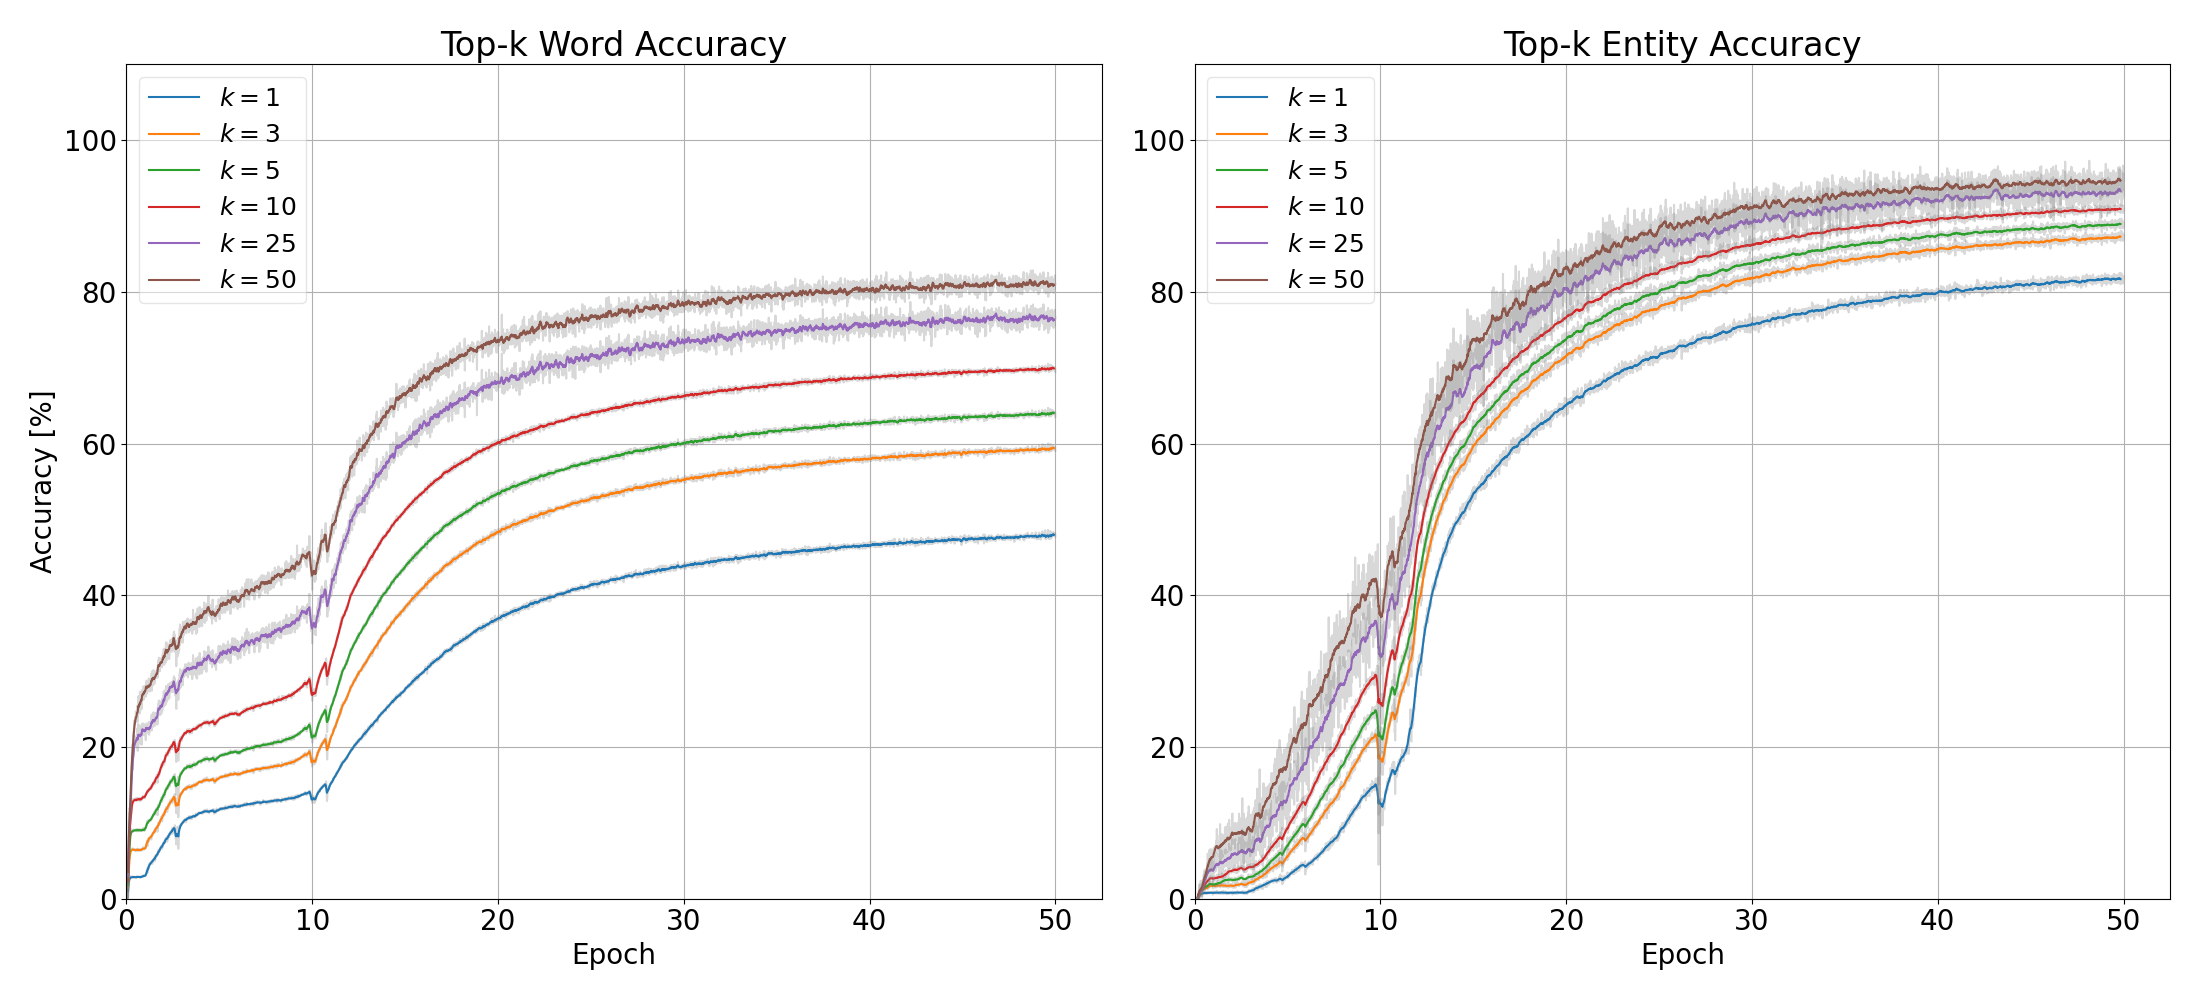
\includegraphics[width=\linewidth]{nobert-acc.png}
    \caption{Development of the masked word and entity accuracies during the course of the pretraining without initializing from da-BERT weights.
    All curves are smoothed using a rolling average.}
    \label{fig:nobert-acc}
\end{figure}\noindent
This result is unintuitive in that a model scoring highly on \emph{both} masking tasks can underperform on NER.
While the running fine-tuning presented in Section~\ref{subsec:effmore} showed partial decoupling between entity masking and NER results, this result further raises the issue of the model overfitting on the limited dataset even though the masking of words and entities is dynamic.

Thus, the transfer learning from da-BERT clearly turns out to be a help here.
From Figure \ref{fig:nobert-acc}, the initialization seems to provide two things other than initial MLM accuracy:
\begin{itemize}
    \item A regulazation effect that prevents the model from overfitting to the dataset.
    \item Increased pretraining stability.
    The accuracy curves contain a number of sudden jumps and drops that are much rarer in other pretrainings.
\end{itemize}
This stabilization effect is supported by the stable distribution of parameters inherited from da-BERT shown at Figures \ref{fig:weight-dist}.
It should be noted that because no weights came from da-BERT, no weights were ever locked throughout the pretraining in this experiment.
A similar experiment with weights unlocked and initialization from da-BERT showed pretraining accuracies much closer to the baseline, indicating that the reguralizing effect is indeed the use of da-BERT.
\begin{enumerate}
    \item Lav et appendiks-afsnit til dette eksperiment
\end{enumerate}

\subsection{Entity Vocabulary Size}
\label{subsec:entvocexp}
For the English LUKE, Yamada et al. used an entity vocabulary of the $500\ctp3$ entities \cite[Sec. 3.4]{yamada2020luke}m even though the English Wikipedia contains $\sim 6\ctp6$ content pages\footnotemark.
\footnotetext{English Wikipedia Statistics: \url{https://en.wikipedia.org/wiki/Special:Statistics}. Visited March 3, 2021.}
This is, apart from crude filtering of non-entity pages, a result of cutting the entity domain down to the most frequent hyperlinks.
For the Danish Wikipedia, however, the number of content pages\footnotemark is $\sim 267\ctp3$ resulting in the DaLUKE entity vocabulary containing $\sim 225\ctp3$ entities.
\footnotetext{Danish Wikipedia Statistics: \url{https://da.wikipedia.org/wiki/Speciel:Statistik} Visited March 3, 2021.}
As this is a much smaller world of entities, the entity vocabulary of the main DaLUKE model was not cut by frequency.

An experiment was performed where entities that were mentioned less than 50 times were excluded from the data, resulting in a vocabulary of $19,119$ entities.
This was done on the augmented data explained in Section \ref{sec:dawiki}.
After pretraining for 50 epochs with the same hyperparameters as the main experiment, the following performance was observed.

\begin{table}[H]
    \centering
    \footnotesize
    \begin{tabular}{l|l|cccccc}
        Model                                 & Top $k$ accuracy [\pro]  & $k=1$  & $k=3$ & $k=5$ & $k=10$ & $k=25$ & $k=50$\\\hline
        \multirow{2}{*}{Limited entity vocab.}& Masked words             & 23.9  & 30.5 & 33.9 & 39.2  & 47.1  & 53.0 \\
                                              & Masked entities          & 30.6  & 42.2 & 48.9 & 55.8  & 65.9  & 66.3
    \end{tabular}
    \caption{
        The top $k$ accuracy of the entity vocabulary-limited model in the 50'th and last epoch.
    }
    \label{tab:few-ents-acc}
\end{table}\noindent
The performance on the word prediction task is slightly worse for this entity vocabulary experiment, while clearly higher scores are seen on the masked entity task.
As for the data augmentation experiment, attention must again be put on the changes in the benchmark itself;
the accuracy of 31\pro\ is calculated in a $\sim 20\ctp3$ class problem while the baseline accuracy of 29\pro\ is calculated over almost ten times as many classes.

% 2021-06-11 19:38:47.989    INFO        K=1
%                                        Word:   23.905
%                                        Entity: 30.585
% 2021-06-11 19:38:47.998    INFO        K=3
%                                        Word:   30.500
%                                        Entity: 42.149
% 2021-06-11 19:38:48.005    INFO        K=5
%                                        Word:   33.902
%                                        Entity: 47.872
% 2021-06-11 19:38:48.011    INFO        K=10
%                                        Word:   39.185
%                                        Entity: 55.786
% 2021-06-11 19:38:48.017    INFO        K=25
%                                        Word:   47.108
%                                        Entity: 65.914
% 2021-06-11 19:38:48.022    INFO        K=50
%                                        Word:   53.028
%                                        Entity: 73.347

The NER performance of this model was, following the approach in the previous experiments, found to be quite close to the performance of the baseline with an average F1 0.2\pro\ points worse.

\begin{table}[H]
    \centering
    \small
    \begin{tabular}{l|ccccc|c|c}
        \multirow{2}{*}{Model}  & \multicolumn{5}{c|}{F1 [\pro]} & Precision [\pro]               & Recall [\pro]               \\
                            & Avg. & LOC & PER & ORG & MISC      & Avg.                           & Avg.                         \\ \hline
    Limited entity vocab.   & 82.2 $\pm 3$ &89.6&93.5&74.0&68.7      & 85.0                          & 79.5
    \end{tabular}
    \caption{The fine-tuning results of the entity vocabulary limiting pretraining experiment.}
    \label{tab:ent-limit}
\end{table}\noindent
% 2021-06-11 15:26:30.316    INFO                      precision    recall  f1-score   support
%                                                 LOC     0.8878    0.9062    0.8969        96
%                                                MISC     0.7358    0.6446    0.6872       121
%                                                 ORG     0.7986    0.6894    0.7400       161
%                                                 PER     0.9385    0.9333    0.9359       180
%                                           micro avg     0.8506    0.7957    0.8222       558
%                                           macro avg     0.8402    0.7934    0.8150       558
%                                        weighted avg     0.8455    0.7957    0.8188       558
Conclusively, the results of this experiment are close to the baseline, signifying robustness in the approach.
However, with these hyperparameters, the removal of entities does not seem promising for the Danish dataset.

This experimental filtering of the DaLUKE entities preserves $7\pro$ of the content pages, while $8\pro$ were preserved for the English LUKE.
Intuitively, it would make sense that the same proportional filtering works better in English, as the absolute number of entities making up the implicit knowledge base of the model might be important:
Smaller datasets, corresponding to smaller language areas, do not equate a smaller shared worlds of named entities.

\subsection{Summary} \label{subsec:preoverview}
Table \ref{tab:mlmsummary} and \ref{tab:nersummary} show the masked language and entity modeling results and fine-tuning results, respectively, of all the just discussed experiments for easier comparison.
\begin{table}[H]
    \centering
    \footnotesize
    \begin{tabular}{l|l|cccccc}
        Model                                 & Top $k$-accuracy [\pro]  & $k=1$  & $k=3$ & $k=5$ & $k=10$ & $k=25$ & $k=50$\\\hline
        \multirow{2}{*}{Baseline}             & Masked words             & 24.2  & 30.9 & 34.4 & 39.7  & 47.7  & 53.6 \\
                                              & Masked entities          & 28.8  & 39.0 & 50.6 & 50.6  & 59.6  & 66.3 \\\hline
        \multirow{2}{*}{BERT attention}       & Masked words             & 20.6  & 26.3 & 29.4 & 34.6  & 42.4  & 48.7 \\
                                              & Masked entities          & 12.3  & 21.0 & 25.7 & 32.8  & 42.9 & 51.5 \\\hline
        \multirow{2}{*}{No data aug.}         & Masked words             & \underline{25.3}  & \underline{32.2} & \underline{35.6} & \underline{40.9}  & \underline{48.8}  & \underline{54.6} \\
                                              & Masked entities          & \underline{34.0}  & 42.9 & 47.2 & 53.5  & 62.3 & \underline{68.8} \\\hline
        \multirow{2}{*}{No transfer learning} & Masked words             & \bfseries 47.9  & \bfseries 59.3 & \bfseries 63.92& \bfseries 69.8  & \bfseries 76.5  & \bfseries 81.0 \\
                                              & Masked entities          & \bfseries 81.7  & \bfseries 87.2 & \bfseries 88.9 & \bfseries 90.9  & \bfseries 93.2 & \bfseries 94.6 \\\hline
        \multirow{2}{*}{Limited entity vocab.}& Masked words             & 23.9  & 30.5 & 33.9 & 39.2  & 47.1  & 53.0 \\
                                              & Masked entities          & 30.6  & \underline{42.2} & \underline{48.9} & \underline{55.8}  & \underline{65.9}  & 66.3
    \end{tabular}
    \caption{
        Overview of final pretraining results for all the experiments presented previously.
        Best result for each metric is shown in boldface with second best result underlined (motivated by quite boring distribution of bests).
    }
    \label{tab:mlmsummary}
\end{table}

\begin{table}[H]
    \centering
    \footnotesize
    \begin{tabular}{l|ccccc|c|c}
        \multirow{2}{*}{Model}  & \multicolumn{5}{c|}{F1 [\pro]} & Precision [\pro]               & Recall [\pro]               \\
                            & Avg. & LOC & PER & ORG & MISC      & Avg.                           & Avg.                        \\ \hline
    Baseline                & 82.4 $\pm 3$&89.5&92.9&74.4&68.8      & \textbf{86.7}                          & 78.4                       \\
    BERT attention          & 79.6 $\pm 3$& 85.8 & 92.8 & 70.9 &   64.8      & 84.5                          & 75.2 \\
    No data augmentation    & \textbf{83.0} $\pm 3$&84.4&\textbf{95.1}&\textbf{76.4}&\textbf{72.1}      & 85.4                          & \textbf{80.8}                       \\
    No transfer learning    & 71.0 $\pm 4$&79.5&83.5&55.4&61.7      & 76.9                          & 65.9                       \\
    Limited entity vocab.   & 82.2 $\pm 3$&\textbf{89.6}&93.5&74.00&68.7      & 85.0                          & 79.5
    \end{tabular}
    \caption{
        Overview of the pretraining experiment fine-tuning results presented in the previous subsections.
        Many of the differences are small and within the $95\pro$ finite sample margin of error, so the performance must be judged in conjunction with masked task performance.
    }
    \label{tab:nersummary}
\end{table}

\section{Fine-tuning Performance}
\label{sec:fine-tuning-exp}
\begin{enumerate}
    \item Statistiske metoder til sammenligning af scores
\end{enumerate}
As with pretraining, fine-tuning has a number of interesting elements that are worth investigating further.
For these experiments, the main pretrained model from section \ref{sec:Pretraining of DaLUKE} are used but with the optimized fine-tuning hyperparameters from Table \ref{tab:main-hyper}.
Following the pretraining experiments, all results are reported with MISC.

\subsection{Stability of LUKE Fine-tuning}
\label{sec:luke-stability}

\paragraph{Reproducability of English LUKE}
For the reproduction of the English LUKE, our results were initially underwhelming as five repetitions of the fine-tuning of LUKE large on CoNLL-2003 consistently, slightly underperformed the reported result of 94.3\pro\ micro average as seen at Table \ref{tab:EnLUKE-wrong}.
This disappointment was backed up by an approximate 95\pro\ confidence interval on the true mean of the avg. F1 score being marginally below the reported value\footnotemark.
\footnotetext{
    Using the one sample Student $t$-based confidence interval relying on an unchecked normality assumption on means, \cite[Method 3.9]{brockhoff2018stat} our five repetitions yield a 95\pro\ confidence interval of $[92.53\pro, 94.26\pro ]$.
    To conclude a significant difference, more repetitions are necessary, but we were initially worried by this result.
}

After investigating, this, to us, somewhat surprising result was revealed to be overturned when fine-tuning with Python version 3.6 and PyTorch 1.2 instead of using newer versions as done in the initial run.
Using these correct versions, the same as Yamada et al. reported in their package file, our results were much closer to the reported numbers as shown in Section \ref{sec:English LUKE Reproduction}.

All in all, the slight hiccups in reproducing the fine-tuning results show the difficulties in empiric evaluations of deep methods strongly relying on indeterminism -- especially as the underlying framework, PyTorch, does not guarantee reproducable results across versions and platforms, even if using identical seeds for the random number generator \cite{pytorchrep}.
\begin{table}[H]
    \centering
    \small
    \begin{tabular}{l l | c c c c c}
            Model & Over 5 repetitions &Micro avg. & LOC & PER & ORG & MISC \\
            \hline
            \multirow{2}{*}{LUKE large}& Mean F1 [\pro] & $93.4$ & $95.2$ & $97.2$ & $93.5$ & $85.2$\\
                                       & Std. [\pro]    & $0.07$ & $0.2$ & $0.08$ & $0.2$ & $0.4$
    \end{tabular}
    \caption{
        Results when pretraining and evaluating LUKE with Python version 3.8 and PyTorch 1.4.
        Using these software versions, the model underperforms reported accuracy slightly.
    }
    \label{tab:EnLUKE-wrong}
\end{table}

\paragraph{Random number generation variance}
The same repetition of the fine-tuning procedure as carried out for English LUKE is done for the main DaLUKE model by training with five different random number generation (RNG) seeds.
The results are shown in Table \ref{tab:seeds}.

              % precision    recall  f1-score   support

         % LOC     0.8632    0.8542    0.8586        96
        % MISC     0.8370    0.6364    0.7230       121
         % ORG     0.8417    0.7267    0.7800       161
         % PER     0.9651    0.9222    0.9432       180

   % micro avg     0.8876    0.7921    0.8371       558
   % macro avg     0.8767    0.7849    0.8262       558
% weighted avg     0.8842    0.7921    0.8338       558

              % precision    recall  f1-score   support

         % LOC     0.7963    0.8958    0.8431        96
        % MISC     0.7890    0.7107    0.7478       121
         % ORG     0.8015    0.6522    0.7192       161
         % PER     0.9222    0.9222    0.9222       180

   % micro avg     0.8390    0.7939    0.8158       558
   % macro avg     0.8273    0.7952    0.8081       558
% weighted avg     0.8368    0.7939    0.8122       558

              % precision    recall  f1-score   support

         % LOC     0.8776    0.8958    0.8866        96
        % MISC     0.7963    0.7107    0.7511       121
         % ORG     0.8264    0.7391    0.7803       161
         % PER     0.9438    0.9333    0.9385       180

   % micro avg     0.8693    0.8226    0.8453       558
   % macro avg     0.8610    0.8198    0.8391       558
% weighted avg     0.8665    0.8226    0.8433       558
              % precision    recall  f1-score   support

         % LOC     0.7961    0.8542    0.8241        96
        % MISC     0.7727    0.7025    0.7359       121
         % ORG     0.7801    0.6832    0.7285       161
         % PER     0.9535    0.9111    0.9318       180

   % micro avg     0.8384    0.7903    0.8137       558
   % macro avg     0.8256    0.7877    0.8051       558
% weighted avg     0.8372    0.7903    0.8121       558

              % precision    recall  f1-score   support

         % LOC     0.8454    0.8542    0.8497        96
        % MISC     0.7925    0.6942    0.7401       121
         % ORG     0.7823    0.7143    0.7468       161
         % PER     0.9432    0.9222    0.9326       180

   % micro avg     0.8498    0.8011    0.8247       558
   % macro avg     0.8408    0.7962    0.8173       558
% weighted avg     0.8473    0.8011    0.8230       558
\begin{table}[H]
    \centering
    \begin{tabular}{l|ccccc|c|c}
        \multirow{2}{*}{Seed}  & \multicolumn{5}{c|}{F1 [\pro]} & Precision [\pro]               & Recall [\pro]               \\
                            & Avg. & LOC & PER & ORG & MISC      & Avg.                           & Avg.                        \\ \hline
     1                      & 83.7&85.8&94.3&78.0&72.3  & 88.7                          & 79.2                        \\
     2                      & 81.5&84.3&92.2&71.9&74.7  & 83.9                          & 79.3                       \\
     3                      & 84.5&88.6&93.8&78.0&75.1  & 86.9                          & 82.2                       \\
     4                      & 81.3&82.4&93.1&72.8&72.8  & 83.8                          & 79.0                       \\
     5                      & 82.4&84.9&93.2&74.6&74.0  & 84.9                          & 80.1                       \\\hline
     Mean                   & 82.7& 85.2& 93.3& 75.0& 73.8& 85.6& 80.0\\
     Std.                   & 1.4& 2.3& 0.8& 2.8& 1.2& 2.1& 1.3
    \end{tabular}
    \caption{Repeating the fine-tuning procedure of the main model, reporting results.}
    \label{tab:seeds}
\end{table}\noindent
Unfortunately, the standard deviation is rather large compared to the margins between many of the experiments.
For reference, seed 1 was used for all experiments bar this one.
The stochasticity of the fine-tuning procedure, possibly driven by the limited size of the training set, casts doubt on NER comparisons.
As Table \ref{tab:seeds} shows, one of the models (seed 3) actually achieves state of the art.

\paragraph{Dataset split variance}
Another way to look at fine-tuning indeterminism is by the randomness in dataset.
Predefined splits, chosen randomly by the dataset creators at the Alexandra Institute \cite{hvingelby2020dane}, into training, development and testing datasets were used for all experiments.
A less noisy estimate of generalization performance is generally obtained by $K$-fold cross validation as opposed to this simple hold-out testing method \cite[Sec. 1.3]{bishop2006pattern}.
This is performed using $K=5$ random splits as this gives a training set of approximately the same size as for the predefined splits, that is, 4383 examples in the DaNE splits and 4410 in cross validation training.
The cross validation test sets will thus be larger, as no development set is used.

 % ┆   ┆   LOC     0.9111    0.9193    0.9152       223
 % ┆   ┆  MISC     0.8740    0.8301    0.8515       259
 % ┆   ┆   ORG     0.8235    0.8273    0.8254       220
 % ┆   ┆   PER     0.9573    0.9458    0.9515       332

 % ┆ micro avg     0.8980    0.8859    0.8919      1034
 % ┆ macro avg     0.8915    0.8806    0.8859      1034
% weighted avg     0.8980    0.8859    0.8918      1034

 %              precision    recall  f1-score   support

 % ┆   ┆   LOC     0.8682    0.8819    0.8750       254
 % ┆   ┆  MISC     0.8651    0.7842    0.8226       278
 % ┆   ┆   ORG     0.7935    0.7300    0.7604       200
 % ┆   ┆   PER     0.9569    0.9284    0.9424       335

 % ┆ micro avg     0.8822    0.8425    0.8619      1067
 % ┆ macro avg     0.8709    0.8311    0.8501      1067
% weighted avg     0.8812    0.8425    0.8610      1067

 %                  precision    recall  f1-score   support

 % ┆   ┆   LOC     0.9031    0.8913    0.8972       230
 % ┆   ┆  MISC     0.8717    0.8208    0.8455       240
 % ┆   ┆   ORG     0.8051    0.7336    0.7677       214
 % ┆   ┆   PER     0.9281    0.9435    0.9357       301

 % ┆ micro avg     0.8836    0.8558    0.8695       985
 % ┆ macro avg     0.8770    0.8473    0.8615       985
% weighted avg     0.8818    0.8558    0.8682       985

 %                  precision    recall  f1-score   support

 % ┆   ┆   LOC     0.9087    0.9045    0.9066       220
 % ┆   ┆  MISC     0.8000    0.7850    0.7925       214
 % ┆   ┆   ORG     0.8232    0.8011    0.8120       186
 % ┆   ┆   PER     0.9416    0.9508    0.9462       305

 % ┆ micro avg     0.8780    0.8714    0.8747       925
 % ┆ macro avg     0.8684    0.8604    0.8643       925
% weighted avg     0.8772    0.8714    0.8742       925
 %              precision    recall  f1-score   support

 % ┆   ┆   LOC     0.9071    0.9111    0.9091       225
 % ┆   ┆  MISC     0.8273    0.8240    0.8257       250
 % ┆   ┆   ORG     0.8136    0.7682    0.7903       233
 % ┆   ┆   PER     0.9506    0.9565    0.9536       322

 % ┆ micro avg     0.8813    0.8718    0.8765      1030
 % ┆ macro avg     0.8747    0.8650    0.8696      1030
% weighted avg     0.8802    0.8718    0.8759      1030

% Micro avg. F1 estimate
% 0.8749122627819783
\begin{table}[H]
    \centering
    \begin{tabular}{l|ccccc|c|c}
        \multirow{2}{*}{Split}  & \multicolumn{5}{c|}{F1 [\pro]} & Precision [\pro]               & Recall [\pro]               \\
                            & Avg. & LOC & PER & ORG & MISC      & Avg.                           & Avg.                        \\ \hline
                    1    &  89.1 & 91.5 & 95.1 & 82.5 & 85.1 & 89.8 & 88.5\\
                    2    &  86.1 & 87.5 & 94.2 & 76.0 & 82.2 & 88.2 & 88.1\\
                    3    &  86.9 & 89.7 & 93.5 & 76.7 & 84.5 & 88.3 & 85.5\\
                    4    &  87.4 & 90.6 & 94.6 & 81.2 & 79.2 & 87.8 & 87.1\\
                    5    &  87.6 & 90.9 & 95.3 & 79.0 & 86.9 & 88.1 & 87.1\\\hline
                    Mean &  87.4 & 90.0 & 94.5 & 79.1 & 83.6 & 88.4 & 87.3\\
                    Std. &  1.1  & 1.6 & 0.7 & 2.8& 3.0 & 0.8 & 1.7
    \end{tabular}
    \caption{
        5-fold cross validation results over the DaNE dataset.
        The training, dev. and test sets were all combined and then split in five different ways with each split having 80\pro\ training data and 20\pro\ test data, on which the F1 score is calculated.
    }
    \label{tab:cross}
\end{table}\noindent
These results at Table~\ref{tab:cross} imply that the DaNE testing set performance of 82.89\pro\ understates the accuracy of this method.
An explanation can be that the small testing set (565 sentences) simply contains more difficult examples than other parts of the dataset.
This theory is substantiated by the differing distributions of entities between DaNE splits (testing contains fewer LOC's and more ORG's, see Figure~\ref{fig:dadatadist}) and that we consistently observed higher performance on the development set than on the testing (such as in the hyperparameter optimization results at Table~\ref{tab:hyperres}).

It must be noted that we cannot claim to present an unbiased estimate of the generalization performance, even on datasets following the same distribution, as the main experiment hyperparameters, that were also used here, were chosen based on performance on much of the data.
\paragraph{Dataset generalization ability}
It was noted in the results section that DaLUKE appears to generalize well to the two other Danish NER datasets.
To add detail to the ability to generalize across these three datasets, DaLUKE is also fine-tuned for the two other datasets and the results for each model is reported across datasets at Table~\ref{tab:datasets}.
\begin{table}[H]
    \centering
    \footnotesize
    \begin{tabular}{l l | c c c c | c c c c}
        \multirow{2}{*}{Test set} & \multirow{2}{*}{Model trained on} & \multicolumn{4}{c|}{Micro Avg. [\pro]} & \multicolumn{4}{c}{Class F1 [\pro]}\\
                    &         & F1    & Prec. & Rec. & F1 {\tiny\textdiscount MISC} & LOC   & PER   & ORG   & MISC \\\hline
            DaNE    & DaNE    & 82.8 & 84.6 & 81.1 & 85.1                   & 87.0 & 94.1 & 73.1 & 74.5 \\
            DaNE    & Plank   & 69.0 & 60.5 & 80.2 & 78.8                   & 81.6 & 92.5 & 56.0 & 13.2 \\
            DaNE    & WikiANN &  --  & -- & -- & 66.8                       & 73.4 & 74.8 & 44.1 & -- \\\hline
            Plank   & DaNE    & 63.4 & 80.8 & 52.1 & 73.1                   & 76.0 & 90.4 & 45.6 & 4.6 \\
            Plank   & Plank   & 74.9 & 78.0 & 72.0 & 74.9                   & 76.2 & 90.3 & 50.5 & 41.0 \\
            Plank   & WikiANN &  --  & -- & -- & 58.4                       & 62.8 & 74.6 & 21.3 & -- \\\hline
            WikiANN & DaNE    &  --  & -- & -- & 67.8                       & 67.9 & 87.5 & 51.2 & -- \\
            WikiANN & Plank   &  --  & -- & -- & 60.5                       & 68.5 & 88.0 & 29.2 & -- \\
            WikiANN & WikiANN &  --  & -- & -- & 93.4                       & 93.4 & 94.7 & 88.3 & --
    \end{tabular}
    \caption{
        Results when fine-tuning and evaluating across datasets.
        Results without the MISC categories are included as WikiANN does not include this category.
    }
    \label{tab:datasets}
\end{table}\noindent
As the table shows, generalizability is not a given.
While some LOC and PER generalize fairly well between datasets, ORG, and especially MISC, see very poor performance when evaluated on another dataset than the model was fine-tuned on.
One cause for this may be the different distributions of labels between datasets.
Another is that the understanding of what the entity categories actually cover.
WikiANN is automatically annotated and so is obviously different from the human-annotated DaNE and Plank, where human language understanding played a role.
However, as DaNE and Plank have different annotations, clearly the authors had different interpretations of what the categories meant (as is especially clear with the MISC category), even though both used the CoNLL-2003 guidelines.
These issues cast doubt on the generalizability of NER.
\cite{hvingelby2020dane, plank2019neural, pan2017wikiann, tjang2003conll}

\subsection{Class-weighted Loss}
\label{subsec:lossexp}
Cross entropy loss weighted by the number of training examples in each class was speculated to improve performance on the class-imbalanced NER task in which 99.3\pro\ of spans are not entities.
In the hyperparameter search, all combinations of learning hyperparameters were also tried with this weighting of loss defined in formula \eqref{eq:w-crossentropyloss}.
From the results at Table~\ref{tab:hyperres}, no general improvement could be seen when weighting and the best combinations were slightly worse when using this approach.
However, two experiments with suboptimal hyperparameters of high learning rate, high dropout, and low weight decay resulted in the model degenerating to predicting the positive entity classes much too often as seen from Table~\ref{tab:clsgood}.
Interestingly, this problem was mitigated when using class-weighted loss, an unintuitive result in our estimation as we expected this weighting to motivate more positive predictions.

\begin{table}[H]
    \footnotesize
    \begin{tabular}{lllll|rrr}
        Batch size & Learning rate & Weight decay & Dropout & Loss weight & F1    &  Precision & Recall\\\hline
        8& 5\ctp{-5}& 0.01& 0.1& Yes         & 84.9 &  80.4 &  90.0\\
        8& 5\ctp{-5}& 0.01& 0.1& No          & 31.5 &  19.8 &  76.4\\
        16& 5\ctp{-5}& 0.01& 0.1& Yes        & 82.6 &  76.8 &  89.3\\
        16& 5\ctp{-5}& 0.01& 0.1& No         & 29.2 &  18.0 &  76.0
    \end{tabular}
    \caption{
        The only hyperparameter search experiments in which class-weighted loss clearly improved performance.
        The unweighted experiments suffer from very high recall and low precision, corresponding to many false positives.
    }
    \label{tab:clsgood}
\end{table}\noindent
Conclusively, this idea did not benefit our main results, a testament to the robustness of gradient learning, but gave an example of how strategies for class imbalance can be necessary when the learning is less stable.

\subsection{Feature Usage}%
\label{sub:Feature Usage}
An entity candidate forward passed through the final, classifying layer in the NER model is comprised of the concatenation of word representations of first and final subword tokens, and, novelly for LUKE, a contextual representation of the entity span.
Two fine-tuning experiments are performed by altering this entity feature approach by observing the performance when the subword token and entity representations are used individually.

\begin{table}[H]
    \centering
    \footnotesize
    \begin{tabular}{l|ccccc|c|c}
        \multirow{2}{*}{Model}  & \multicolumn{5}{c|}{F1 [\pro]} & Precision [\pro]               & Recall [\pro]               \\
                       & Avg.           & LOC            & PER            & ORG            & MISC           & Avg.           & Avg.  \\ \hline
        Subword tokens & 81.2         $\pm 3$ & \textbf{87.6} & 92.4          & 70.9          & 71.6          & 84.6          & 78.1 \\
        Entity tokens  & 81.7         $\pm 3$ & 85.1          & 93.2          & 71.4          & 74.0          & \textbf{85.0} & 78.6 \\
        Both (default) & \textbf{82.8}$\pm 3$ & 87.0          & \textbf{94.1} & \textbf{73.1} & \textbf{74.5} & 84.6          & \textbf{81.1}
    \end{tabular}
    \caption{
        Fine-tuning results using different features for the classifier.
        Best results are marked in bold.
    }
    \label{tab:concat}
\end{table}\noindent
From the results shown at Table~\ref{tab:concat}, it is learned that the model is able to perform the NER task with high performance using any of the three feature combinations.
This is explainable by both entities and words interacting with each others representations in the transformer and thus affecting the final representations given to the classifier no matter how these are chosen.
The combination of both representation types seems to outperform the others though this might be due to the high RNG variance.

The experiment where only the entity tokens are used is arguably a simple and more elegant NER approach as the selection of the first and last subword tokens to describe a span seems arbitrary.
These results make such an approach seem to be viable.


\section{Predictions: What Is Learned?}
Until this point, we have used the benchmark performance to judge the models.
To get a better understanding of the model, this section includes attempts to introspectively interpret the model predictions.

\subsection{Masked Language Predictions}
\label{subsec:mlmpreds}
To demonstrate DaLUKE's ability to consider context, an example, and some variations on it, are constructed.
The example is given below with text sequence first, followed by entity annotations.
\begin{itemize}
    \item ''[MASK] blev angrebet af USA i 2003 som følge af terrorangrebet den 11. september 2001. Saddam Hussein blev fanget i december.''
    \item[] Truth: ''Irak''
    \item $\{$ \emph{[MASK]} at word \#1,
            \subitem \emph{USA} at word \#5,
            \subitem \emph{2003} at word \#6,
            \subitem \emph{Terrorangrebet den 11. september 2001} at words \#11-15,
            \subitem \emph{Saddam Hussein} at words \#12-13
        $\}$
    \item[] Truth: ''Irak''.
\end{itemize}
First consider the shorter version: "[MASK] blev angrebet af USA i 2003 som følge af terrorangrebet d. 11. september 2001."
Given this text piece, DaLUKE predicts "afghanistan"\footnote{Model predictions are lower-cased, as the da-BERT tokenizer is lower-cased.} with a certainty of 15.95\pro.
While certainly a reasonable guess, it is incorrect, as Afghanistan was attacked in 2001.
For context, "irak" is the second guess of the model with 4.98\pro\ certainty.
Furthermore, the masked "Irak" entity is predicted as "USA", but only with 7.61\pro~certainty.
Adding the additional context of Saddam Hussein being captured, however, makes DaLUKE predict "irak" with 17.64\pro~certainty.
Furthermore, the masked "Irak" entity is predicted as "Irak" with 15.57\pro~certainty.

This example highlights how DaLUKE is able to take advantage of context to substantially improve its predictions.
The following examples show similar results.
For simplicity, no entities are annotated.
\begin{itemize}
    \item "I [MASK] spises der meget and." -- "danmark" is predicted, which makes perfect sense but was not "december" as was first intended with the sentence.\\
    "I [MASK] spises der meget and. Det er nemlig julemåneden." -- "december" is now predicted.
    \item "Danmarks vigtigste lov er [MASK]." -- "bekendtgørelser", which while grammatically correct does not make much sense in the context.\\
    "Danmarks vigtigste lov er [MASK]. Den blev underskrevet i 1849." -- "grundloven" is correctly predicted.
\end{itemize}


\subsection{DaLUKE Representations: The NER Geometry}
DaLUKE produces contextualized representations of both words and entities and these were, for the NER task, successfully adapted to show a level of language understanding.
These abstract representations which, ideally, condense language understanding into 768 reals are here subjected to some examination.
The entity span representations, the concatenation of contextual word and entity representations $\mathbf v_i \in \RR^{2304}$, are analysed by conducting DaLUKE inference on every possible span in the DaNE training data, and saving each result, thus producing a sequence of representations $\mathbf v_{1, \ldots, 975312}$.
The pretrained, but not fine-tuned model was used.
Dimensionality reduction for visualization on the representations was performed using principal component analysis (PCA), the $t$-SNE ($t$-distributed stochastic neighbour embedding) algorithm \cite{maaten2008tsne} and the UMAP (uniform manifold approximation and projection for dimensionality reduction) algorithm \cite{mcinnes2020umap}.

Implementation wise, Sci-Kit Learn was used for $t$-SNE \cite{pedregosa2011scikit} and UMAP Learn was used for UMAP \cite{mcinnes2018umap-software} with hyperparameters shown on Table~\ref{tab:dimreducer-hyper}.
The set of 975,312 entity spans in the DaNE training set was randomly subsampled to 100K examples for these non-linear dimensionality reduction algorithms due to compute limitations.
Even with this limit and with hyperparameters chosen to favour global structure, $t$-SNE and UMAP results were difficult to interpret, see Appendix~\ref{sec:dimredu}, motivating visualizing the dataset where only the 4,003 entity spans that corresponded to true entity annotations were included.

\begin{table}[H]
    \centering
    \begin{tabular}{l|r}
        Parameter           &  Value\\\hline
        $t$-SNE perplexity  &  1,000   \\
        UMAP $N$ neighbours &  300\\\hline
        \multicolumn{2}{c}{When only including positives}\\\hline
        $t$-SNE perplexity  & 100\\
        UMAP $N$ neighbours & 50
    \end{tabular}
    \caption{
        The hyperparameters used for the dimensionality reduction algorithms run on the DaLUKE entity representations.
        All other hyperparameters followed the defaults in Sci-Kit Learn 0.24.1 and UMAP Learn 0.5.1.
    }\label{tab:dimreducer-hyper}
\end{table}\noindent
Dimensionality reduction on the full dataset yields weakly structured visualizations of the geometry, mostly dominated by giant clusters, as seen for PCA at Figure \ref{fig:all-pca}, which also shows some clustering of true entities, and at the others in Appendix~\ref{sec:dimredu}.
The true, underlying dimensionality of the representations also seems high as the first 100 principal components only explain less than 60\pro\ of data variance, see Figure \ref{fig:full-varex}, an indication of well-learned representations which, ideally, should exploit all vector coordinates by having minimal latent dimension covariance.

\begin{figure}[H]
    \centering
        \includegraphics[width=0.7\linewidth]{full-geo/pca_matrix}
    \caption{
        The first four components visualized against each other from PCA performed on all 975,312 possible entity spans in the DaNE training data.
        Spans in grey are annotated entities in the dataset.
        The non-entity spans are more dispersed, intuitively making sense when considering that these include all possible spans of words only limited by the maximum length of 16 subword tokens.
    }
    \label{fig:all-pca}
\end{figure}\noindent
For the reductions in the positive label-only dataset, even more meaningful structure is apparent with all three methods, at Figures \ref{fig:pos-pca}, \ref{fig:pos-tsne}, \ref{fig:repvslen}, showing slight grouping of entities in the same NER class, indicating that the pretrained model, even before fine-tuning, represents language in a way that is close to the human annotated dataset.

\begin{figure}[H]
    \centering
        \includegraphics[width=0.7\linewidth]{pos-geo/pca_matrix}
    \caption{
        The first four components visualized against each other from PCA performed on only the 4,003 entity spans that are annotated to a NE class in the DaNE training data.
        Class separation is observed in multiple of the components, exemplifying why the NER classification problem is solved well by DaLUKE which only requires few epochs to distinguish classes.
    }
    \label{fig:pos-pca}
\end{figure}\noindent

\begin{figure}[H]
    \centering
        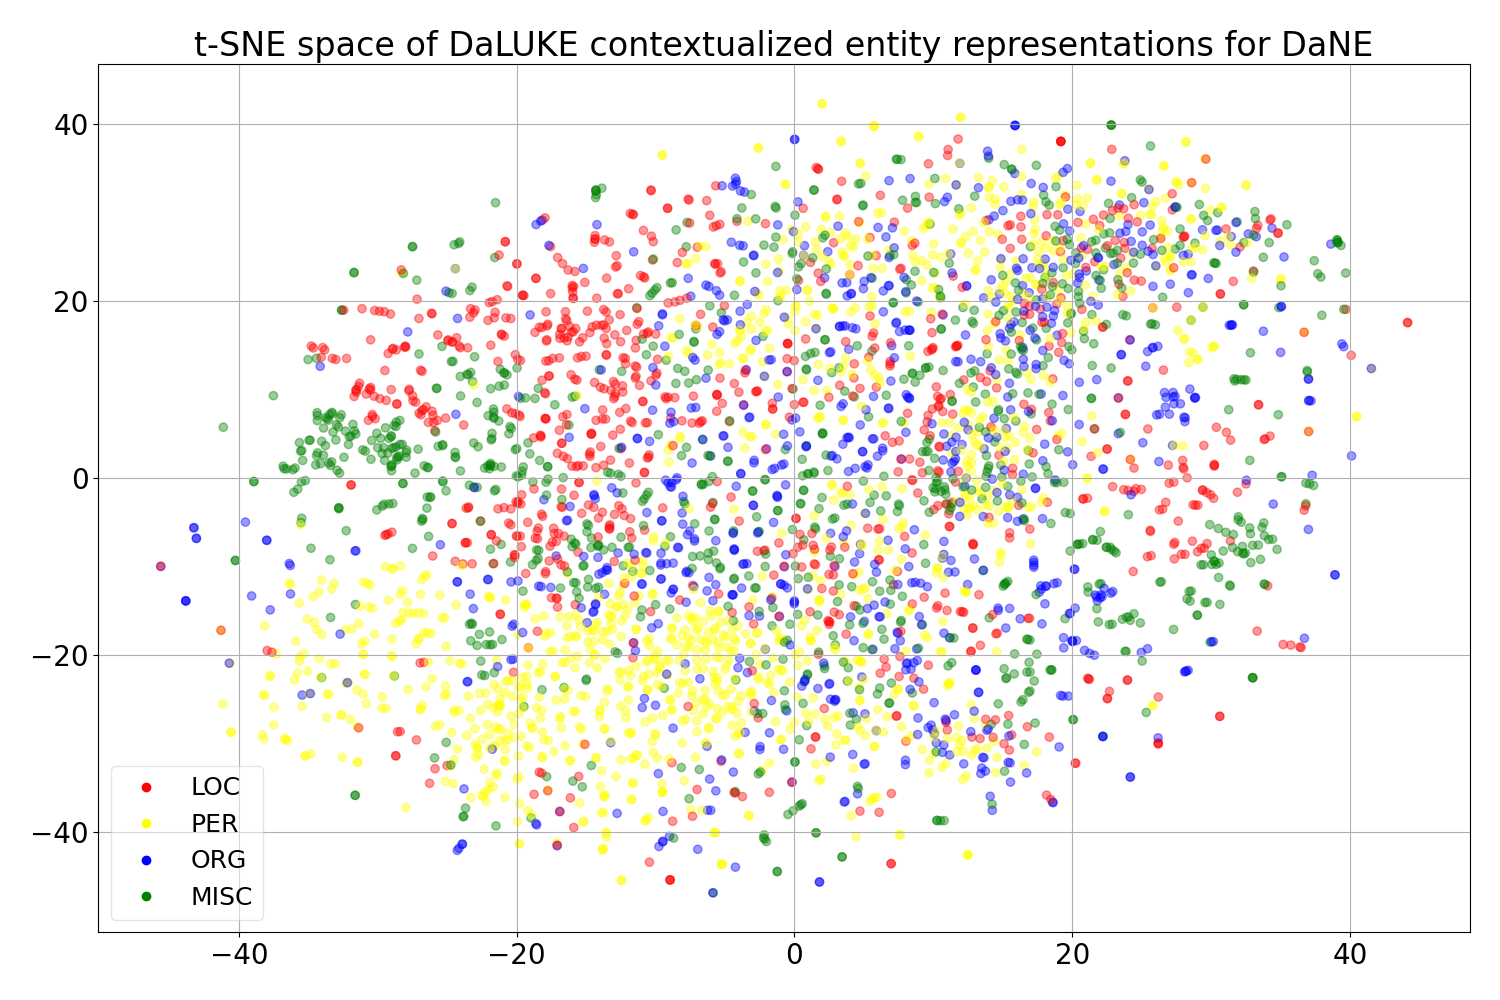
\includegraphics[width=0.495\linewidth]{pos-geo/tsne}
        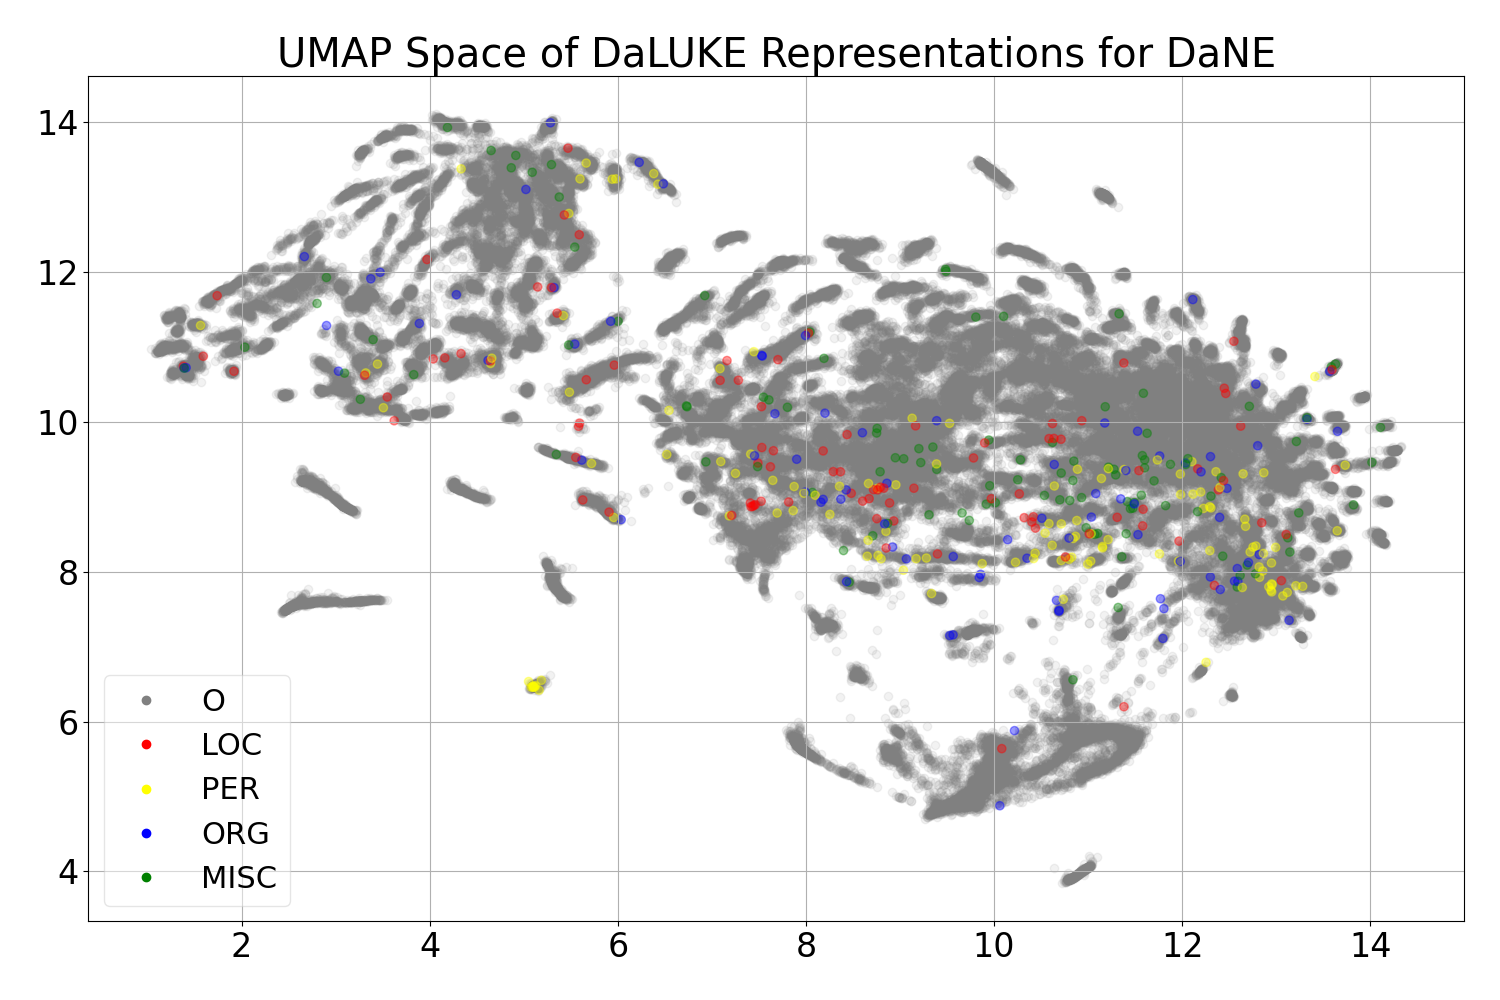
\includegraphics[width=0.495\linewidth]{pos-geo/umap}
    \caption{
        $t$-SNE and UMAP projections of the DaNE dataset containing entity spans with positive labels.
        While the classes are not strongly separated, some clusters consisting of mostly one class are clearly visible in both projections.
    }
    \label{fig:pos-tsne}
\end{figure}\noindent
The obvious question is what these plots mean: What do the clusters and the dimensions themselves correspond to?
This is far from a trivial task; while it is possible to correlate the dimensionality reduced coordinates to the original dimensions, more clever thinking is required to correlate both to human language understanding.
We mostly leave this task for further work, but perform a case-based inspection of the predictions.
Our qualitative observations are summarized below with supporting examples in Table~\ref{tab:dimexamples}.
\begin{itemize}
    \item
        The second principal component in the dataset including all data seems to express something related to span position, as the highest values in this dimension almost all correspond to examples with the span at the very end of the sentence.
        Based on this, it makes sense that the plots in Figure~\ref{fig:all-pca} shows the actual entities having moderate values.
    \item
        Low values of the fourth principal component in the positive-label only dataset seems to correspond to a very specific type of words:
        Adjectivizations of political, geographic regions such as "Danish" or "English".
        As explained in Section~\ref{subsec:annoschemes}, such entities should have the label MISC.
        This observation fits with Figure~\ref{fig:pos-pca} showing MISC generally having the lowest 4th dimension values and LOC coming in second.
    \item
        For $t$-SNE on the positive-only dataset, no such clear dependencies on coordinate numeric values were observed, explainable by $t$-SNE not returning linear projections, but an approximate recreation of data point distances.
        Two examples very close in $t$-SNE distances are shown in Table~\ref{tab:dimexamples}; these are also semantically very similar in entity type and role.
    \item
        For UMAP fitted to the examples with positive labels, the clear cluster placed around $\left( -2.5, 7\right)$ is examined.
        Here, every entity is revealed to a derivative of the word \emph{Danmark}.
        Some of these are MISC (adjectivizations, demonyms) and some LOC (\emph{Danmark} itself) as seen at Figure~\ref{fig:pos-tsne}.
\end{itemize}
\begin{table}[H]
    \footnotesize
    \centering
    \begin{tabularx}{\linewidth}{llclX}
        Data    & Alg.      & Vector                     & \jl{Class}  & Example \\\hline

        Full    & PCA       & $\begin{bmatrix}-11.75\\\underline{36.44}\\-4.85\\16.42\\\vdots\end{bmatrix}$ & O           & De følgende 10 år er der ydet omkring 800 mio. kr. til enkeltprojekter \textbf{og forskningsinstitutter}.\\[3em]

        Full    & PCA       & $\begin{bmatrix}-8.78\\\underline{32.14}\\-1.64\\14.64\\\vdots\end{bmatrix}$ & LOC           & Den syriske leder ankom i går til Abu Dhabi efter besøg i Saudi-Arabien og \textbf{Kuwait}.\\[3em]

        % Full    & PCA       & $\begin{bmatrix}-0.50\\\underline{-11.53}\\-1.78\\5.66\\\vdots\end{bmatrix}$ & O           & Også i Baku \textbf{syntes der at} være roligere, selv om soldater i pansrede køretøjer og lastbiler patruljerede i gaderne, og der var demonstrationer i centrum af byen, oplyste en talsmand for det aserbajdsjanske udenrigsministerium.\\

        Positives    & PCA       & $\begin{bmatrix}-0.23\\-5.63\\-9.60\\\underline{-15.17}\\\vdots\end{bmatrix}$ & MISC        & Det \textbf{jugoslaviske} præsidentråd appellerede i sidste øjeblik til FN om at undlade at iværksætte en boykot og opfordrede til, at der i stedet indkaldes til en international konference om konflikten.\\

        Positives    & PCA       & $\begin{bmatrix}2.30\\5.32\\4.91\\\underline{-13.13}\\\vdots\end{bmatrix}$ & MISC        & Med indsættelse af \textbf{europæiske} fartøjer rykker Vestunionen for første gang i centrum af europæisk sikkerhed efter mange års debat om at lette USAs byrder ved forsvaret af Europa.\\

        Positives    & $t$-SNE       & $\begin{bmatrix}\underline{-37.77}\\-22.41\end{bmatrix}$ & PER        & "Piloten forsøgte at rette maskinen op -- så kunne jeg ikke se mere, men pludselig var der gnister i luften," siger øjenvidnet \textbf{Peter de Neef}.\\

        Positives    & $t$-SNE       & $\begin{bmatrix}\underline{-37.75}\\-22.36\end{bmatrix}$ & PER        & "Løfterne om bonus har jeg heller aldrig fået svar på, hvor bare en undskyldning kunne have gjort underværker," understreger \textbf{Peter Freil}.\\

        Positives    & UMAP       & $\begin{bmatrix}-2.54\\\underline{7.27}\end{bmatrix}$ & MISC       & Datoen for den dag i april, da han fik sin tro på det \textbf{danske} retssystem tilbage.\\

        Positives    & UMAP       & $\begin{bmatrix}-2.07\\\underline{7.17}\end{bmatrix}$ & LOC        & Roskilde Domkirke bliver 12. november rammen om den første af en række koncerter, den norske sangerinde Sissel Kyrkjebø giver i \textbf{Danmark}.

\end{tabularx}
    \caption{
        \footnotesize
        Selected entity examples chosen for having high values in resulting dimensions.
        An example consists of a sentence and an entity candidate -- the example entity span is here visualized with boldface words.
        The coordinate value which is extreme and motivated the inclusion of the example is underlined.
    }
    \label{tab:dimexamples}
\end{table}\noindent

Furthermore, a key quality of the representations is their contextualized nature; this is shown to be present in the reduced dimensions, as multiple of these are correlated with the length of the example sequence as shown in Figure~\ref{fig:repvslen}.

\begin{figure}[H]
    \centering
        \includegraphics[width=0.495\textwidth]{full-geo/PCA0-sequence-len}
        \includegraphics[width=0.495\textwidth]{pos-geo/PCA0-sequence-len}
        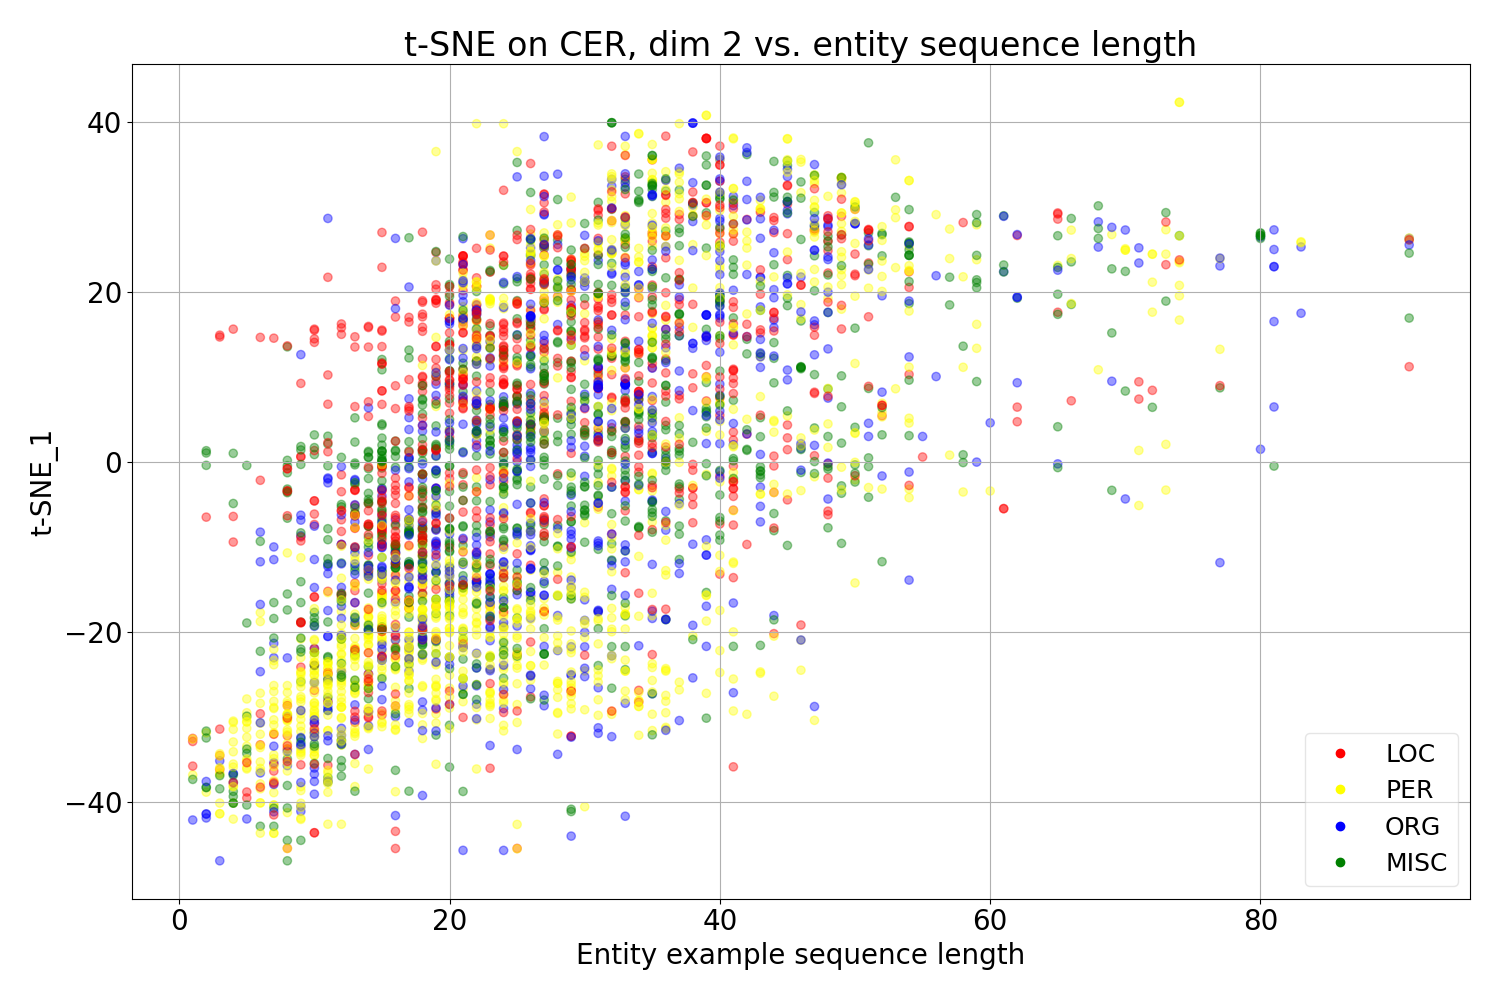
\includegraphics[width=0.495\textwidth]{pos-geo/t-SNE1-sequence-len}
        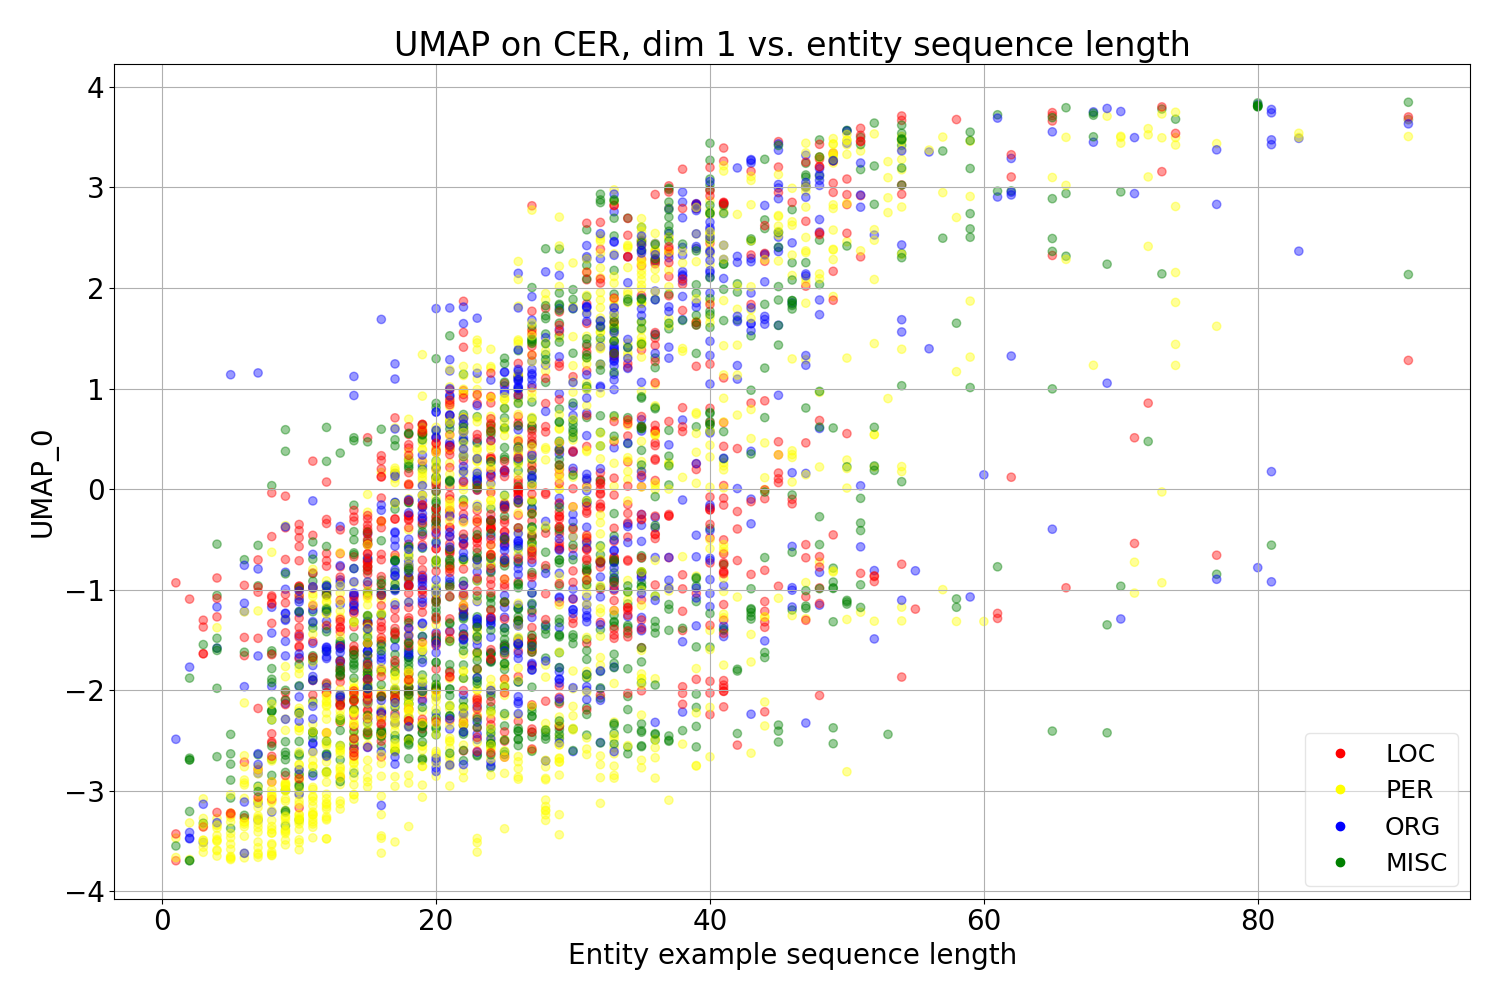
\includegraphics[width=0.495\textwidth]{pos-geo/UMAP0-sequence-len}
     \caption{
        Four selected reduced dimensions, the first (top left) from the full dataset and the three others from the dataset only containing positives, visualized as a function of the length of the sentence that the entity example appears in.
    }
    \label{fig:repvslen}
\end{figure}\noindent

\subsection{When the Model is Wrong}

Analysing when the model is right or wrong may provide valuable insight into how the classification decisions are made and how to improve this.
For this reason, a confusion matrix (Table \ref{tab:pred-true-confmat}) is constructed for the DaNE testset that shows predicted labels against the true labels\footnotemark.
\footnotetext{
    All confusion matrices in this section are for simplicity and nuance done on the word level and not on entire entity span level.
    This means that these confusion matrices do not correspond exactly to the reported precision and recall scores, as these were calculated on span level as explained in Section~\ref{subsec:nereval}.
}

%      | O    | LOC | PER | ORG | MISC
%-----+------+-----+-----+-----+-----
%O    | 9197 | 5   | 0   | 8   | 14
%LOC  | 5    | 91  | 0   | 2   | 3
%PER  | 5    | 0   | 307 | 3   | 3
%ORG  | 21   | 23  | 11  | 154 | 12
%MISC | 29   | 0   | 0   | 16  | 114

\begin{table}[H]
    \centering
    \small
    \begin{tabular}{l l | r r r r r }
        & &	\multicolumn{5}{c}{Predicted label}	\\
        \multirow{5}{*}{True label} & & LOC & PER & ORG & MISC & O \\\hline
            & LOC  & 91 & 0    & 2   & 3   & 5   \\
            & PER  & 0  & 307  & 2   & 3   & 5   \\
            & ORG  & 23 & 11   & 154 & 12  & 21  \\
            & MISC & 0  & 0    & 16  & 114 & 29  \\
            & O    & 5  & 0    & 8   & 14  & 9,197
    \end{tabular}
    \caption{
        Predicted labels versus the true labels on the DaNE test set.
        Note that this count is done on word level, so entities spanning multiple words appear multiple times in the table.
    }
    \label{tab:pred-true-confmat}
\end{table}\noindent
From the table, there are two major sources for errors:
\begin{enumerate}
    \item LOC is often erroneously predicted on ORG entities -- but not the other way around.
    \item O is often predicted on true labels, especially on ORG and MISC. This results in the relatively low recall of $81.18\pro$ holding back performance compared to the precision of $84.67\pro$.
\end{enumerate}
Point 1 may have a relatively simple explanation: 
That many organizations are named after a geographic location while locations more rarely adopts the name of an organization.
Consider for instance the organization entity "Bakken" in the (verbatim) test example: ''Alle som én er en hyldest til Bakken.''.

The model predicts LOC, but while the amusement park, Bakken, would refer to the physical location in another context, this sentence is about an homage to the tradition of the park as an institution and is as such marked as ORG.
While the model is contextual, meaning correctly predicting such entities is possible, examples with as little context as this one requires a degree of very minute real world knowledge currently not obtained by DaLUKE.
This error pattern also occurred with names of theatres, libraries and municipalities.
\begin{table}[H]
    \footnotesize
    \begin{tabular}{l|llllllllll}
        Text:   & Nørrebro  & Bibliotek  & introducerede  &for  &et  &par  &år  &siden  &NU-bøgerne & $\ldots$ \\
        Truth:  & B-ORG     & I-ORG      & O              &O    &O   &O    &O   &O      &B-MISC  & $\ldots$    \\
        Pred.:   & B-LOC     & I-LOC      & O              &O    &O   &O    &O   &O      &O   & $\ldots$\\\hline
    \end{tabular}\par
    \begin{tabular}{l|llllllll}
        Text:    & $\ldots$  &Folkekongressen  &skal  &give  &præsidenten  &diktatoriske  &beføjelser  &.\\
        Truth:   & $\ldots$  &B-ORG            &O     &O     &O            &B-MISC        &O           &O\\
        Pred.:   & $\ldots$  &O                &O     &O     &O            &O             &O           &O\\\hline
    \end{tabular}\par
    \begin{tabular}{l|llllllll}
        Text:    & $\ldots$ &  om  &Landsforeningen  &Ungbo  &har  &begået  &mandatsvig  & $\ldots$ \\
        Truth:   & $\ldots$ &  O   &B-ORG            &I-ORG  &O    &O       &O           & $\ldots$ \\
        Pred.:   & $\ldots$ &  O   &O                &B-ORG  &O    &O       &O           & $\ldots$
    \end{tabular}
    \caption{
        Example sentences where DaLUKE is wrong, including conflating an organization with its location, missing cased and adjective entities, and greedily selecting a subspan instead of the full entity.
    }
    \label{tab:dalukeerrors}
\end{table}\noindent
Point 2, the prevalence of false negatives (prediction case III, following table~\ref{tab:eval}), can be a calibration problem,
%as examined in CALIBRATION,
but is also, in our estimation, one of the most difficult parts of this dataset, as the definition of named entities starts becoming quite murky.
One common cause found is the model missing a number of adjectives marked as MISC including ''borgerlig'', ''indremissionsk'' and ''olympisk''.
The classification of these as named entities with the MISC label is correct following CoNLL-2003 definition (see Section~\ref{subsec:annoschemes}) but we speculate that this might be a difference in language understanding between English and Danish as this categorization, in our estimation, seems non-intuitive in Danish -- in which adjectives are also never capitalized.

In the missed organizations, two possible causes are found.
Firstly, using a case-sensitive tokenizer, which the da-BERT is not \cite{botxo2019dabert}, might help some errors such as ''Markedsudvalget'' and ''Kulturministeriets''.
Secondly, cases such as ''EFs ministerråd'' with the annotation ''B-ORG I-ORG'' are found.
Here, the model only predicts the first word as an organization and gets the entire entity wrong.
As ''EFs'' might follow a pattern more common in the training data than ''EFs ministerråd'', the former has higher estimated probability by the model and is greedily selected.
This tendency to predict subspans highlights a weakness of the method of greedily selecting partially overlapping spans.

From this qualitative impression of the errors, a subset of which are shown in Table~\ref{tab:dalukeerrors}, no smoking gun was found that problematizes this specific model.
Rather, most errors shown here are examples that genuinely are difficult applications of language knowledge.
To get more insight into the prediction patterns of DaLUKE specifically, the NER predictions are compared with those of other Danish NER algorithms.

Initially, the similarity of other model predictions and those of DaLUKE are measured using the proportion of words for which the prediction is the same, shown at Table~\ref{tab:covar}.
Surprisingly, the most similar models are the DaCy models, using the multilingual RoBERTa base and large behind the hood \cite{enevoldsen2020dacy}, and the multilingual BERT from NERDA, while da-BERT, on which DaLUKE is based, follows behind.

\begin{table}[H]
    \centering
    \begin{tabular}{l | c }
        Model               & Same prediction as DaLUKE [\pro]\\\hline
        DaNLP da-BERT       & 97.86\\
        NERDA m-BERT        & 98.44\\
        NERDA Ælæctra       & 97.70\\
        DaCy medium         & 98.68\\
        DaCy large          & \textbf{98.76}\\
        DaNLP spaCy         & 97.65\\
        DaNLP Flair         & 96.37\\
        Polyglot            & 93.45\\
        daner               & 95.90
    \end{tabular}
    \label{tab:covar}
    \caption{
        Co-prediction frequencies between DaLUKE and other Danish NER algorithms on the DaLUKE testing dataset.
        This calculation is performed on the word level.
    }
\end{table}\noindent
Compared to the da-BERT predictions, the biggest difference is the higher amount of positive predictions as seen on Table~\ref{tab:dabertcompare}.
DaNLP da-BERT was not fine-tuned for MISC, so this difference is natural, but DaLUKE also discovers more organizations.
DaLUKE also predicts location more rarely and clearly outperforms da-BERT on these (F1: 87.0\pro\ vs. 83.9\pro).

% 2021-06-19 16:31:04.881    INFO        Confusion matrix with DaLUKE results ↓ and results from BERT-DaNE →
% 2021-06-19 16:58:48.906    INFO             | LOC | PER | ORG | MISC | O
%                                        -----+-----+-----+-----+------+-----
%                                        LOC  | 114 | 0   | 0   | 0    | 5
%                                        PER  | 0   | 310 | 5   | 0    | 3
%                                        ORG  | 10  | 9   | 143 | 0    | 21
%                                        MISC | 1   | 0   | 4   | 0    | 141
%                                        O    | 4   | 3   | 6   | 0    | 9244
\begin{table}[H]
    \centering
    \begin{tabular}{l l | r r r r r }
        & &	\multicolumn{5}{c}{da-BERT predictions}	\\
        \multirow{5}{*}{DaLUKE predictions} & & LOC & PER & ORG & MISC & O \\\hline
        & LOC  & 114 & 0   & 0   &  --    & 5  \\
        & PER  & 0   & 310 & 5   &  --    & 3  \\
        & ORG  & 10  & 9   & 143 &  --    & 21 \\
        & MISC & 1   & 0   & 4   &  --    & 141\\
        & O    & 4   & 3   & 6   &  --    & 9244
    \end{tabular}
    \label{tab:dabertcompare}
    \caption{
        da-BERT predictions vs. DaLUKE predictions.
    }
\end{table}\noindent
From examining the examples where the models differ, DaLUKE seems employ the additional learned knowledge to better disambiguate between similar classes and use context to discover named entities, see Table~\ref{tab:daberterrors}.
% Uddybe mere - det her er jo vores chance for at blære

\begin{table}[H]
    \footnotesize
    \begin{tabular}{l|llllllll}
        Text:             & $\ldots$  & redegørelsen  & i  & det    & udenrigspolitiske  & nævn   & $\ldots$ \\
        Truth:            & $\ldots$  & O             & O  & B-ORG  & I-ORG              & I-ORG  & $\ldots$ \\\hline
        DaLUKE pred.:     & $\ldots$  & O             & O  & B-ORG  & I-ORG              & I-ORG  & $\ldots$ \\
        da-BERT pred.:    & $\ldots$  & O             & O  & O      & O                  & O      & $\ldots$ \\
    \end{tabular}\par
    \begin{tabular}{l|lllllllllllllll}
        Text:            &  "Ih,   & hvor  & jeg  & glæder  & mig  & til  & et  & lille  & glas,"  & lød  & det  & fra  & Lykke  \\
        Truth:           &  O    & O     & O    & O       & O    & O    & O   & O      & O        & O    & O    & O    & B-PER  \\\hline
        DaLUKE pred.:    &  O    & O     & O    & O       & O    & O    & O   & O      & O        & O    & O    & O    & B-PER  \\
        da-BERT pred.:   &  O    & O     & O    & O       & O    & O    & O   & O      & O        & O    & O    & O    & O
    \end{tabular}\par
    \begin{tabular}{l|llllllllllll}
        Text:            & Rapporten  & $\ldots$  & er  & bestilt  & og  & betalt  & af  & Københavns  & Amtsråd  & $\ldots$\\
        Truth:           & O          & $\ldots$  & O   & O        & O   & O       & O   & B-ORG       & I-ORG    & $\ldots$\\\hline
        DaLUKE  pred.:   & O          & $\ldots$  & O   & O        & O   & O       & O   & B-ORG       & I-ORG    & $\ldots$\\
        da-BERT pred.:   & O          & $\ldots$  & O   & O        & O   & O       & O   & B-LOC       & I-LOC    & $\ldots$
    \end{tabular}
    \caption{
    }
    \label{tab:daberterrors}
\end{table}\noindent
The same comparison is made to DaCy Large which achieves higher performance than DaLUKE -- especially driven by improvements in organization and miscellaneous classes.
Here, the biggest differences lies in cases where the models have to discern between these two classes and  null class, seen at Table~\ref{tab:dacycompare}.

% 2021-06-19 16:29:26.614    INFO        Confusion matrix with DaLUKE results ↓ and results from DaCyLarge-DaNE →
% 2021-06-19 16:58:11.740    INFO             | LOC | PER | ORG | MISC | O
%                                        -----+-----+-----+-----+------+-----
%                                        LOC  | 108 | 0   | 2   | 1    | 8
%                                        PER  | 0   | 309 | 6   | 3    | 0
%                                        ORG  | 9   | 3   | 154 | 5    | 12
%                                        MISC | 0   | 1   | 3   | 120  | 22
%                                        O    | 8   | 4   | 8   | 27   | 9210
\begin{table}[H]
    \centering
    \begin{tabular}{l l | r r r r r }
        & &	\multicolumn{5}{c}{DaCy Large predictions}	\\
        \multirow{5}{*}{DaLUKE predictions} & & LOC & PER & ORG & MISC & O \\\hline
           & LOC                             &  108 & 0   & 2   & 1    & 8\\
           & PER                             &  0   & 309 & 6   & 3    & 0\\
           & ORG                             &  9   & 3   & 154 & 5    & 12\\
           & MISC                            &  0   & 1   & 3   & 120  & 22\\
           & O                               &  8   & 4   & 8   & 27   & 9210
    \end{tabular}
    \label{tab:dacycompare}
    \caption{
        DaCy Large predictions vs. DaLUKE predictions.
    }
\end{table}\noindent
Examples where DaCy Large is right, but DaLUKE wrong, are shown at Table~\ref{tab:dacyex}.
The initial explanation of DaCy Large's edge over DaLUKE was the use of a BERT large-sized transformer, adding flexibility to the model, theoretically allowing higher level language features to be learned compared to the base size model used by DaLUKE.
From the examples, more reasons are identified.
One cause is the use of the case sensitive byte-pair encoding tokenizer of RoBERTa \cite{conneau2020unsupervised} which we speculate helps discovering more entities, relating to the high recall of DaCy (83.7\pro versus the 81.2\pro of DaLUKE).
Another interesting pattern lies in the strength of the multilingual model used by DaCy correctly predicting entities in foreign languages.

\begin{table}[H]
    \footnotesize
    \begin{tabular}{l|llllll}
        Text:             & $\ldots$  & opus    & VIII    & der  & hedder  \\
        Truth:            & $\ldots$  & B-MISC  & I-MISC  & O    & O       \\\hline
        DaLUKE pred.:     & $\ldots$  & B-MISC  & I-MISC  & O    & O       \\
        DaCy pred.:       & $\ldots$  & O       & O       & O    & O
    \end{tabular}
    (continued)\\
    \begin{tabular}{c} % The spooky, scary, invisible ghost Table for formatting!
        \quad \quad \quad \quad \quad \quad \quad \quad \quad \quad \quad
    \end{tabular}
    \begin{tabular}{llllll}
            Il      & Cimento  & dell'Armonia  & e       & dell'Invenzione \\
            B-MISC  & I-MISC   & I-MISC        & I-MISC  & I-MISC          \\\hline
            O       & O        & O             & O       & O               \\
            B-MISC  & I-MISC   & I-MISC        & I-MISC  & I-MISC
    \end{tabular}\vspace*{1em}
    \begin{tabular}{l|llllllll}
        Text:             & Der  & ligger  & fire  & skodder  & plus  & en  & hel  & Camel   \\
        Truth:            & O    & O       & O     & O        & O     & O   & O    & B-MISC  \\\hline
        DaLUKE pred.:     & O    & O       & O     & O        & O     & O   & O    & O       \\
        DaCy pred.:    & O    & O       & O     & O        & O     & O   & O    & B-MISC
    \end{tabular}\vspace*{1em}
    \begin{tabular}{l|llllll}
        Text:            & Den  & modtog  & han  & i  & øvrigt  & Kulturministeriets\\
        Truth:           & O    & O       & O    & O  & O       & B-ORG             \\\hline
        DaLUKE  pred.:   & O    & O       & O    & O  & O       & O                 \\
        DaCy pred.:   & O    & O       & O    & O  & O       & B-ORG
    \end{tabular}
    (continued)\\
    \begin{tabular}{c} % The spooky, scary, invisible ghost Table for formatting!
        \quad \quad \quad \quad \quad \quad \quad \quad \quad \quad \quad
    \end{tabular}
    \begin{tabular}{llll}
        børnebogspris  & for  & i  & 1990  \\
        O              & O    & O  & O     \\\hline
        O              & O    & O  & O     \\
        O              & O    & O  & O
    \end{tabular}
    \caption{
        Examples from the DaNE test set where DaCy large gives the correct predictions and DaLUKE gives the wrong predictions.
    }
    \label{tab:dacyex}
\end{table}\noindent

\section{Future Work}
We see promise in this approach of lightly sprinkling some explicit knowledge on top of the model fitting approach for languages such as Danish.
The results are, in our estimation, solid and encouraging.
DaLUKE did not, however, sweep away the classic language modeling approach and was intercepted for the NER crown by the larger model presented in DaCy.
Some parts of the pretraining approach also seemed misguided on the small dataset.
To further understand the DaLUKE performance, the results from other downstream tasks than NER would be of great interest, including coreference resolution on the Dacoref dataset \cite{kromann2004cdt, danlp2021} or dependency parsing on the Danish Dependency Treebank \cite{kromann2003ddt}.
It would also improve the insight to pretrain DaLUKE with a subset of the corpus left out as a testing set.
Some further changes which have the potential to improve performance are proposed.

\paragraph{Data}
As in any deep learning project, we end up crying out for more data.
Multiple of the pretraining experiments presented in Section~\ref{sec:pretrainpls} show signs of the model overfitting to the limited Danish Wikipedia.
An immediate idea is to include the Norweigan Wikipedia as the language (in \emph{bokmål}) is syntactically, and vocabulary wise similar to Danish.
There are some technical issues such as the choice of tokenizer, but also the entity modeling, as the same entity might be spelled differently in both languages.
While the Norwegian Wikipedia has 156M words \footnotemark compared to the 81M of the Danish Wikipedia, this might be too little to dramatically change the results.
\footnotetext{Norwegian Wikipedia statistics: \url{https://no.wikipedia.org/wiki/Spesial:Statistikk}}

A more impactful improvement could be found from our dataset augmentation idea, though it did not improve results for the Danish Wikipedia.
Much needed entirely new LUKE pretraining datasets could be produced from raw text corpora by automatically annotating them using pattern matching.
Such lower standard annotations used to achieve extra data might be necessary for continued improvement in low-resource languages such as Danish but should be used carefully and with an analysis of the trade off between quality and quantity of data.
Other automatic annotaters than simple pattern matching might also be beneficial as the field of entity linking has been applied to Wikipedia \cite{brochier2021wikilink} including ready-to-use tools such as the Danish version of DBpedia Spotlight \cite{isem2013daiber}.
It might hold that the quality of the entity annotations is not all-important, in which case tools that link entire sentences or paragraphs to entities without localizing them exactly might be used.
The entity potition ids could then be omitted.
Here, Danish tools for explicit semantic analysis \cite{hansen2017esa} could help.

The primary, open dataset for which we see promise in automated annotation is the recently published Danish Gigaword corpus which includes documents that are more diverse in domain and dialect than the Danish Wikipedia \cite{derc2021giga}.

Access to closed datasets such as news articles and internal documents could also be a way to increase the available data.
However, such documents are closed for a reason.
In most cases, suppliers of closed documents would have an interest in not risking that these documents could be backwards engineered from the model.
For this, methods such as differential privacy \cite{GONG2020131} could play a role.

Finally, investigating biases in the pretraining dataset could provide insight into why performance is better on some categories than others (see Table \ref{tab:DaNE}).
Obviously, Wikipedia does not categorize articles by the four CoNLL-2003 categories, but many articles are still categorized into larger groups that could light a path to putting all or most articles into the CoNLL boxes.
Such an investigation would be especially important if automatically annotated datasets are incorporated.

\paragraph{Modeling}
Motivated by the impressive success of DaCy, the most direct model improvement is to use the multilingual RoBERTa \cite{conneau2020unsupervised} instead of the Danish BERT \cite{botxo2019dabert}.
The Danish BERT has previously been criticized for being under trained \cite{derc2021giga, nielsen2020textsum} and for not being case-sensitive.
Furthermore, there exists a large version of the multilingual RoBERTa, and, finally, we speculate that our pretraining task will help the multilingual model catch up to possibly missing Danish specific knowledge.
The large version will, however, require more computational resources or more patience.

Further improvement might be found if the LUKE approach is not followed directly.
The LUKE knowledge-enhancement is very subtle and requires any hierarchical and relational modeling of knowledge to be learned implicitly from the flat world of entities stored in the vocabulary.
A unification of models that use subtle knowledge-enhancement in pretraining and those that use explicit knowledge bases might be beneficial for Danish.
An approach to this that maintains a flexible, general model, might be introducing additional tokens coding for knowledge as input for the entity embeddings.
We imagine a hierarchical token that uses the article classification of Wikipedia (see Figure~\ref{fig:wikipedia-cat}) to code the type of token to be beneficial in pretraining.
\begin{figure}[H]
    \centering
    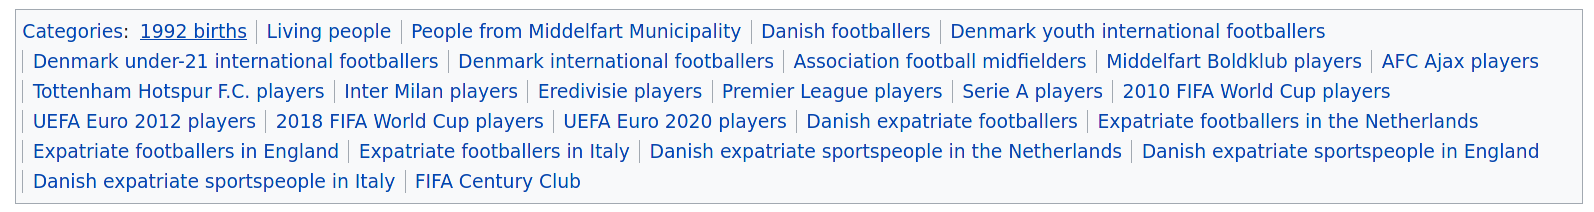
\includegraphics[width=\linewidth]{wikipedia-cat}
    \caption{An example of categories included in Wikipedia articles. It is imagined that these can be mined as additional, helpful annotations of entity types for the pretraining.}
    \label{fig:wikipedia-cat}
\end{figure}\noindent

\paragraph{Ethics}
As with all applications of AI, there are significant ethical concerns.
Hihg-performing language models capable of generating convincing text can be used for automating the production of spam and other deceitful internet content.
For instance, OpenAI claimed that GPT-2 \cite{Radford2019gpt2} generated problematic articles so easily that its release was considerably delayed \footnote{\url{https://www.technologyreview.com/2019/08/29/133218/openai-released-its-fake-news-ai-gpt-2/}. Visited June 26, 20201.}.
Incorporating knowledge in language models might allow bad actors better control over this production, requiring monitoring of the potential harmful consequences of effective NLP.

Another concern is that of unintended offensive or politically charged language.
In order to acquire the amounts of data necessary to train effective language models, many practitioners, including BotXO for da-BERT \cite{botxo2019dabert}, have turned to uncurated web scrapes.
As the internet has no shortage of hate, the models will naturally learn these parts of language.
Such behaviour has for instance been observed with GPT-3 \cite{brown2020language}, the largest language model in existence as of writing\footnote{\url{https://www.technologyreview.com/2020/10/23/1011116/chatbot-gpt3-openai-facebook-google-safety-fix-racist-sexist-language-ai/}. Visited June 26, 2021.}.
One solution could be the use of NLP methods such as hate speech detection, as done for Danish by Sigurbergsson and Derczynski \cite{sigurbergsson-derczynski-2020-offensive}.
However, these problems of language models can also be seen in a larger AI safety context as an alignment problem \cite{taylor2020alignment}:
How do we guarantee that the implicit values of these automated systems are compatible with the our engineering goals of benefiting society?

\end{document}
